\chapter{Supporting Information For Text Analysis}
\label{textappendix}


\section{Introduction}

This appendix presents supporting information for the quantitative analysis sections of Over Pressure: Grassroots-Driven Transformation of (Militant) Organizations. The analysis covers the data selection, processing, and results for a random forest, support vector machine, and t-Distributed Stochastic Neighbor Embedding (t-SNE) clustering of news articles about violence in Yemen attributed to AQAP, Ansar al-Shariah, and the Houthi militant groups. It also describes the data, analysis, and results for a Structural Topic Model of communications from AQAP, Ansar al-Shariah, and as-Sahab.

\section{Media Texts and Processing}

News stories originated in the ICEWS database and were selected by
first querying the database for stories about events located in Yemen. This
resulted in 47,385 stories ranging from January 15, 1991 through January 4,
2015. I selected only \say{violent} events, defined as events that
fall into one of the following ICEWS event types: \say{Threaten with
military force,} \say{Use unconventional violence,} \say{Violate ceasefire,}
\say{Use as human shield,} \say{Threaten,} \say{Occupy Territory,} \say{Physically
assault,} \say{Mobilize or increase armed forces,} \say{Engage in violent
protest for leadership change,} \say{Engage in mass killing,} \say{Conduct
suicide, car, or other non-military bombing,} \say{Carry out suicide
bombing,}\say{Attempt to assassinate,} \say{Assassinate,}\say{Abduct, hijack, or
take hostage,}\say{Fight with small arms and light weapons,} or \say{Fight with
artillery and tanks.}

This resulted in 10,818 stories, of which I took a random sample of
1772 stories. ICEWS codes for event date, event type, source actor,
and target actor. However, the source and target actor codes typically
characterize the actor by their role, such as \say{Armed Rebel} or
\say{Militant,} rather than by group affiliation.

\begin{figure}
\begin{center}
\begin{tabular}{c}
 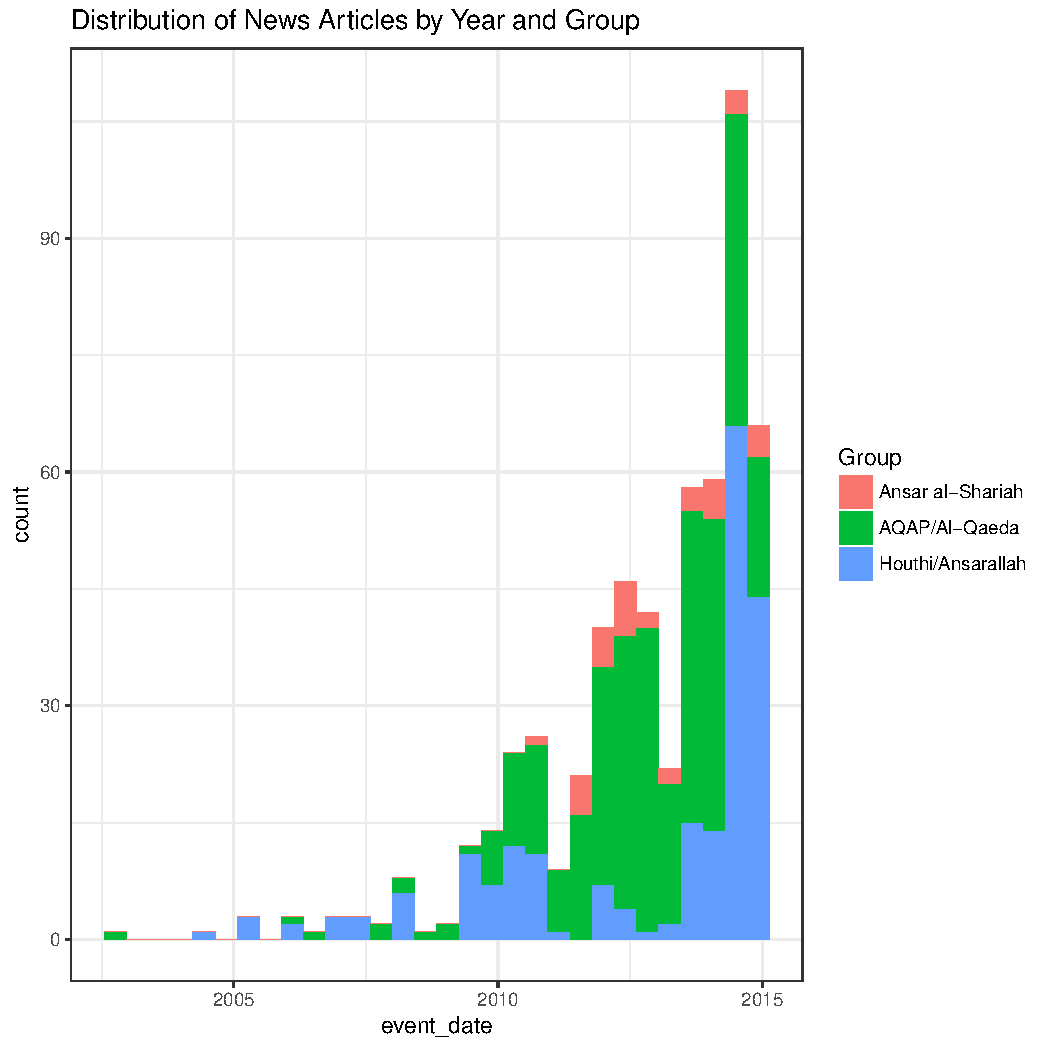
\includegraphics[width=5.00in]{./Pictures/storyHistogram.pdf}
\end{tabular}
\caption{Distribution of News Articles}
\label{fig:news-hist}
\end{center}
 \end{figure}

In order to generate data on how groups operate, I re-coded the reports to include a
variable for group or movement affiliation. I first sent the sample to
Amazon's Mechanical Turk platform, asking the workers to categorize
the stories as relating to an action carried out by Ansar al-Shariah,
AQAP, Houthi/Ansarallah, Yemeni Government, Tribal Uprising, Other,
Multiple Actors, or Unknown.  I kept the tags for the 283 stories that
both coders agreed on, and hand-coded the remaining 1489 stories. The temporal distribution of
the news articles and actor labels can be seen in Figure~\ref{fig:news-hist}. I
then further subset the data to keep only the stories tagged as
describing a violent event carried out by one of the three militias of
interest. This produced the final 720-story corpus of news events.

For each of the development, validation, and test sets, I used the tm() package to tokenize the words in each story and remove numbers, standard English stopwords, whitespace, and stray HTML markup. I additionally removed a custom list of stopwords that strongly signal the group, such as variations on the group name and signifiers of sectarian identity. These custom stopwords are comprised of: words that signal AQAP: \say{qaeda,}\say{alqaida,} \say{alqaeda,} \say{qaida};
words that signaled Houthis: \say{houthi,} \say{huthi,} \say{houthis,} \say{zaidi,} \say{alhouthi}; terms that signaled Ansar al-Shariah: \say{ansar,} \say{sharia,} \say{alsharia};\footnote{The robustness models also remove \say{alshariah} with little change in results.} terms that suggest an al-Qaeda affiliation: \say{laden,}\say{osama}; words often used to summarize location of action for one ofthe groups:\say{peninsula,} \say{northern,} \say{southern,} \say{arabian}\ say{yemen[-]based}; and finally terms that denote sectarian identity: \say{sunni,}\say{shia,}\say{shiite.}\footnote{I did not
remove areas of operation from the texts as the goal of the
classifiers was to seek discussion of operational differences.
Locations of operation are substantively meaningful.}
Word frequency was normalized via term frequency-inverse document frequency (tf-idf), producing a pair
of tf-idf matrices, from which I took the intersection of features
(i.e. words). This generated a set of 2,222 \say{features} for classification in the texts; which reduced the available terms significantly but was necessarily to test models across the training, validation, and test sets.

I reattached metadata to each of the term document matrices. Metadata included group label, date, and whether the
story was coded by Mechanical Turk workers.

The distribution of group labels in the development set can be seen in Table~\ref{tab:dev} with the corresponding distribution from the validation set in Table~\ref{tab:val}.\footnote{Deviations from 100\%
  in the relative frequency sums is due to rounding.}

 \begin{table}
 \centering
 \begin{tabular}{rrr}
   \hline
  & Absolute Frequency & Proportion of Documents \\
   \hline
 Ansar al-Shariah &  27  & 5.8\% \\
   AQAP/Al-Qaeda & 260  & 56.3\%\\
   Houthi/Ansarallah & 174 & 37.7\% \\
   Total & 461 & 99.8\% \\
    \hline
 \end{tabular}
 \caption{Distribution of group labels in development set}
 \label{tab:dev}
 \end{table}

 \begin{table}[ht]
\centering
 \begin{tabular}{rrr}
   \hline
  & Absolute Frequency & Proportion of Documents \\
   \hline
   Ansar al-Shariah & 9 &  7.8\% \\
   AQAP/Al-Qaeda & 67 & 58.2\% \\
   Houthi/Ansarallah & 39 & 33.9\% \\
   Total & 115 & 99.9\% \\
    \hline
 \end{tabular}
 \caption{Distribution of group labels in validation set}
 \label{tab:val}
\end{table}
 
\section{Machine Learning Classifiers}                                                                            
The supervised machine learning techniques used in the paper provide a strategy to adjudicate between the counterfactuals introduced in the theory and qualitative sections. In particular, the clustering analysis indicates that international and local journalists writing
about events in Yemen use similar terms when describing the activities of AQAP and Ansar al-Shariah. This suggests that AQAP has been unable to maintain a local spin-off with a distinctive operational profile. However, one significant caveat is that these techniques are unable to distinguish between AQAP acting like Ansar al-Shariah, Ansar al-Shariah acting like AQAP,\footnote{One natural counterfactual in which an influx of local
  fighters is followed by behavioral convergence of AQAP and Ansar
  al-Shariah but which does not follow the mechanism hypothesized by
  the bottom-up transformation theory could be that AQAP’s
  socialization has been so successful that the group has changed the
  preferences of the communities in which they operate. In this
  scenario, the local Ansar al-Shariah should gain a greater
  international focus as local actors are socialized into the
  transnational jihadi ideology.} or journalists conflating Sunni insurgent
groups. Distinguishing between the three possibilities is important to
assess the theoretical expectation that an inflow of recruits should
pressure AQAP’s leadership to adopt a local emphasis. The topic
modeling section addresses concerns about the direction of convergence.

The following section provides technical details about the
implementation of the t-SNE visualization and the SVM and Random Forest
classifiers.

\subsection{t-SNE Hyperparameter Selection}

Figure~\ref{fig:tSNE}
presents t-SNE clustering for all stories published between 2011 and
2014, presented according to year of publication. These dates provide
a snapshot of writing about each of AQAP (green), Ansar al-Shariah
(red), and the Houthis (blue), and provide a high-level visualization
of the separation or convergence among the words used to describe each
of the three groups. The yearly clustering displayed in~\ref{fig:tSNE} features one point \
per story, and indicates that across the time period, stories about the Houthi insurgency \
appear to be systematically different from stories about the two Sunni groups,
and is suggestive of a pattern in which from 2012 through 2014, the
Ansar al-Shariah stories become progressively more similar to AQAP
stories.

\begin{figure}
  \begin{center}
  \begin{tabular}{ccc}
 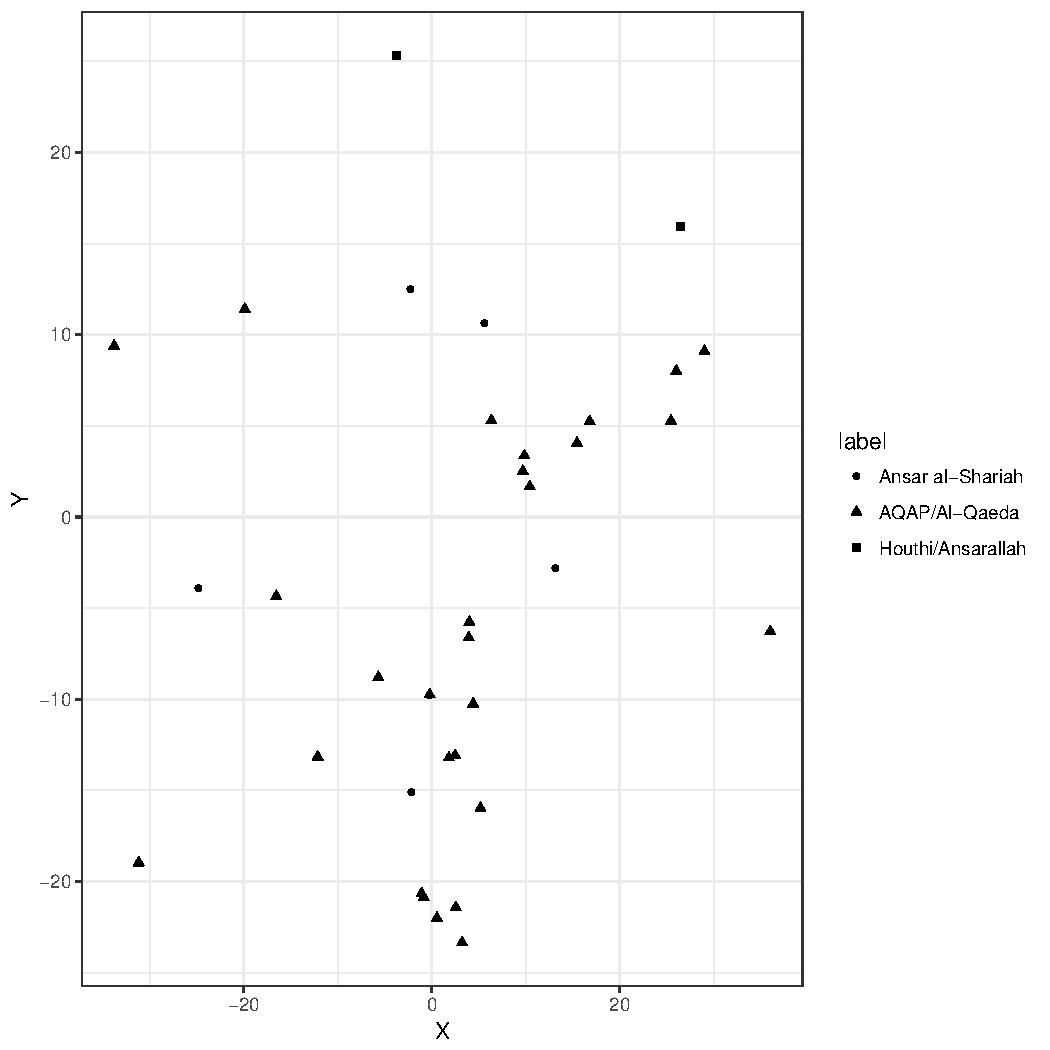
\includegraphics[width=.45\columnwidth]{./Pictures/2011DV_Panel_P50_tSNEDimRed.pdf}&
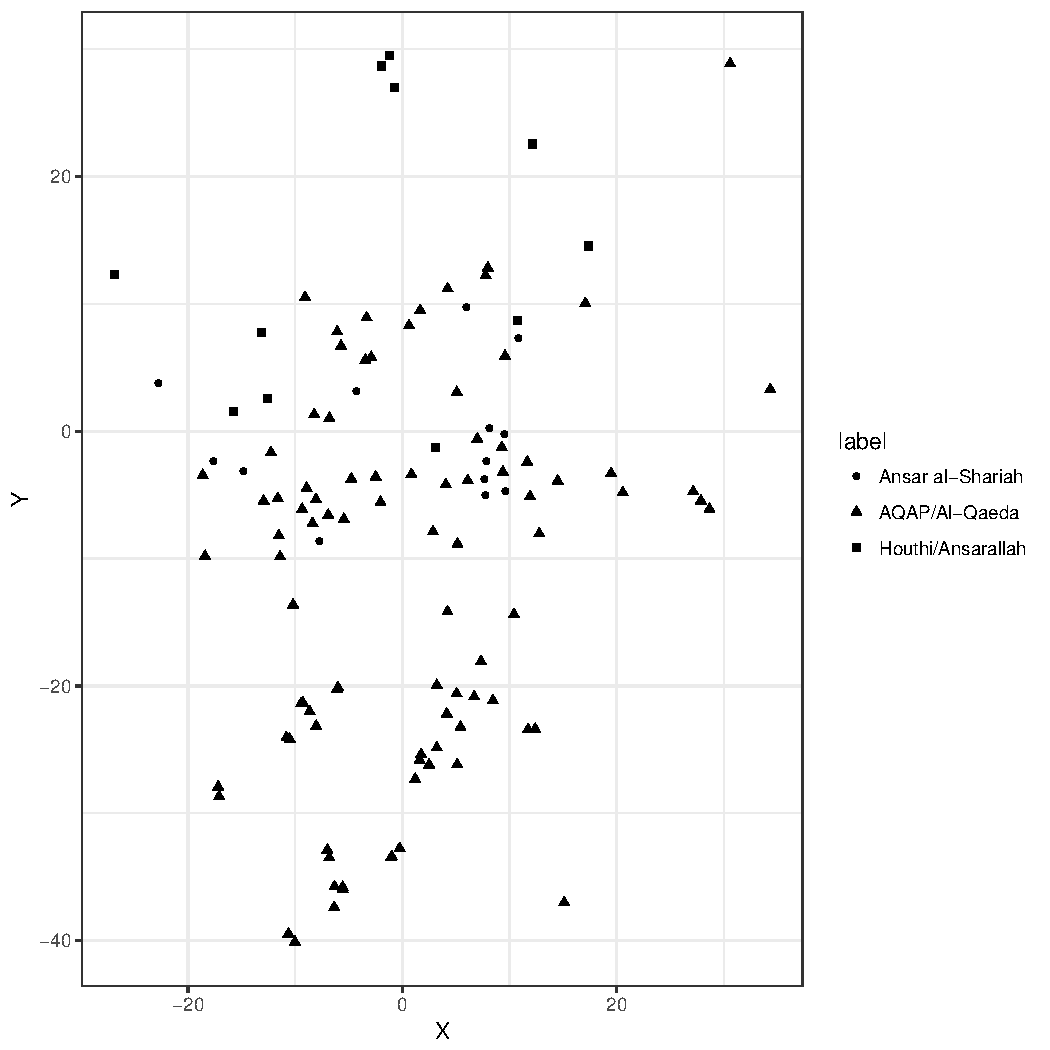
\includegraphics[width=.45\columnwidth]{./Pictures/2012DV_Panel_P50_tSNEDimRed.pdf}\\
 2011 & 2012\\
 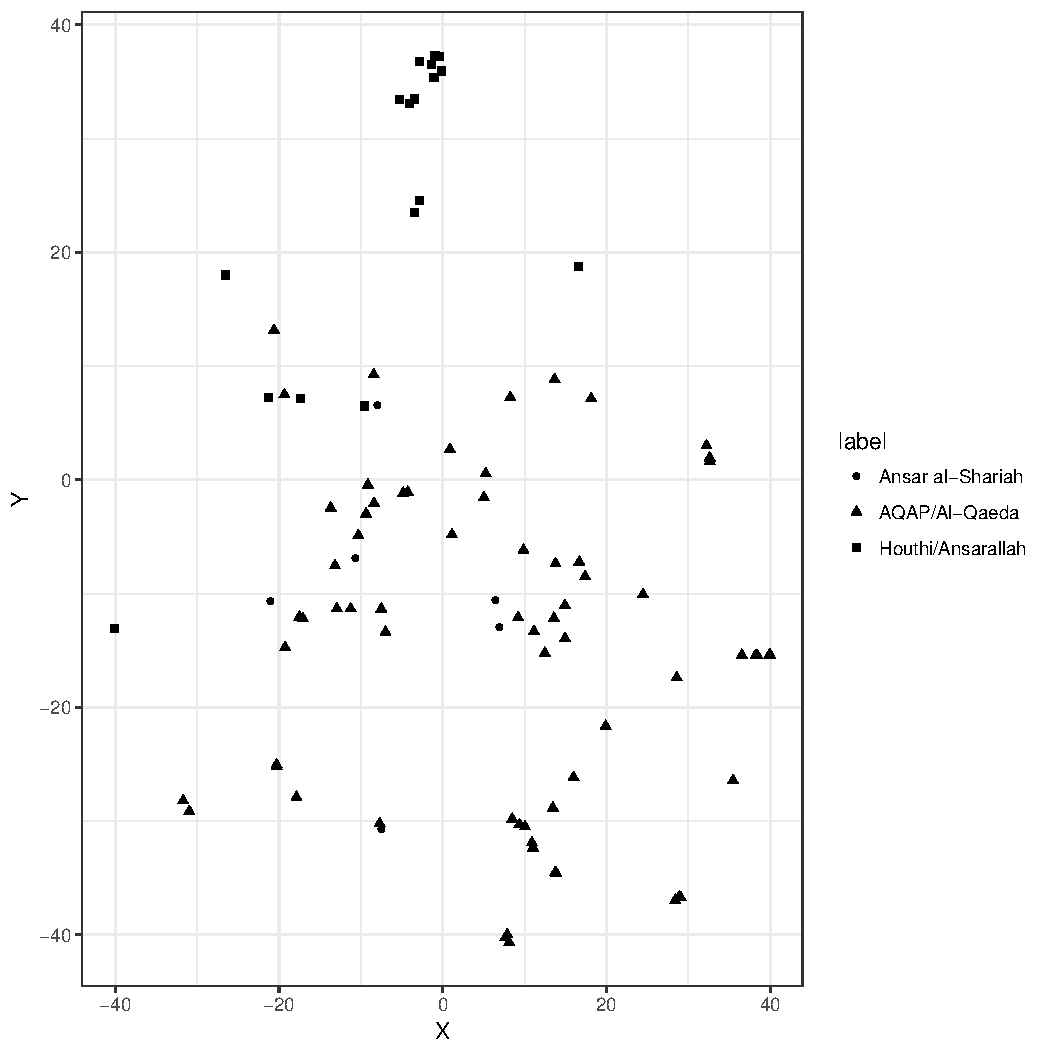
\includegraphics[width=.45\columnwidth]{./Pictures/2013DV_Panel_P50_tSNEDimRed.pdf}&
 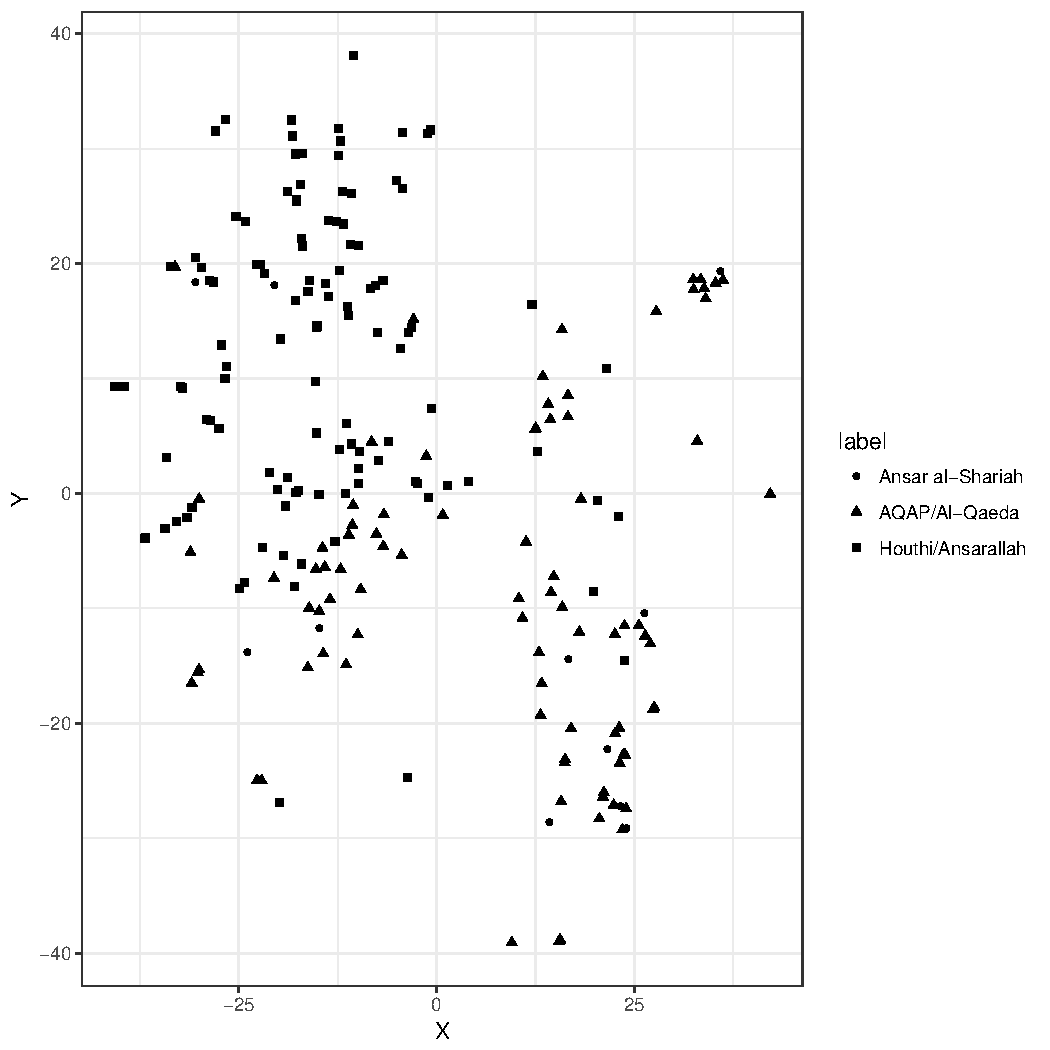
\includegraphics[width=.45\columnwidth]{./Pictures/2014DV_Panel_P50_tSNEDimRed.pdf}\\
  2013 & 2014\\
  \end{tabular}
  \caption{tSNE Clustering, All Stories 2011-2014}
  \label{fig:tSNE}
  \end{center}
  \end{figure}

The visualization presented here was generated by
running the t-SNE algorithm on for 5,000 iterations on the pooled
data. The perplexity hyperparameter presented below was selected after
grid sweeping from 5-50, at intervals of 5. Sweeping the perplexity
hyperparameter changes the exact outcome, as expected from a
probabilistic approach to summarizing structure in complex high
dimensional data, the conclusions are  broadly consistent across the
specifications. To address concerns that the observed clustering is random noise or driven by a specific
initialization, clustering was carried out in parallel on two
different machines using the same specifications but different
starting points. The results were broadly similar, namely  clear separation between the
Sunni and Houthi stories but lack of clear separation among stories
about AQAP and Ansar al-Shariah. As the diffusion and relative
positioning of clusters generated using t-SNE are not inherently
meaningful, comparison across the runs is only impressionistic and
presenting averaged results would not be meaningful.

Figure~\ref{fig:tSNE} presents t-SNE clustering for AQAP and Ansar
al-Shariah stories published between 2011 and 2014, presented
according to year of publication. These dates provide a snapshot of
writing about each of AQAP (green), Ansar al-Shariah (red), and the
Houthis (blue), and provide a high-level visualization of the
separation or convergence among the words used to describe each of the
three groups. The yearly clustering displayed in Figure~\ref{fig:tSNE}
features one point per story, and indicates that across the time
period, stories about the Houthi insurgency appear to be
systematically different from stories about the two Sunni groups, and
is suggestive of a pattern in which from 2012 through 2014, the Ansar
al-Shariah stories become progressively more similar to AQAP stories.
Figure~\ref{fig:tsne-sunnis} focuses only on whether or not the t-SNE
visualization differentiates between Ansar al-Shariah and AQAP
stories. As compared to the separation of the Houthi stories in the
corpus, the two Sunni groups demonstrate no apparent separation. This
implies that stories about the two groups are much more similar than
are stories about AQAP and the Houthi insurgency.   

\begin{center}
\begin{figure}
  \begin{tabular}{cc}
    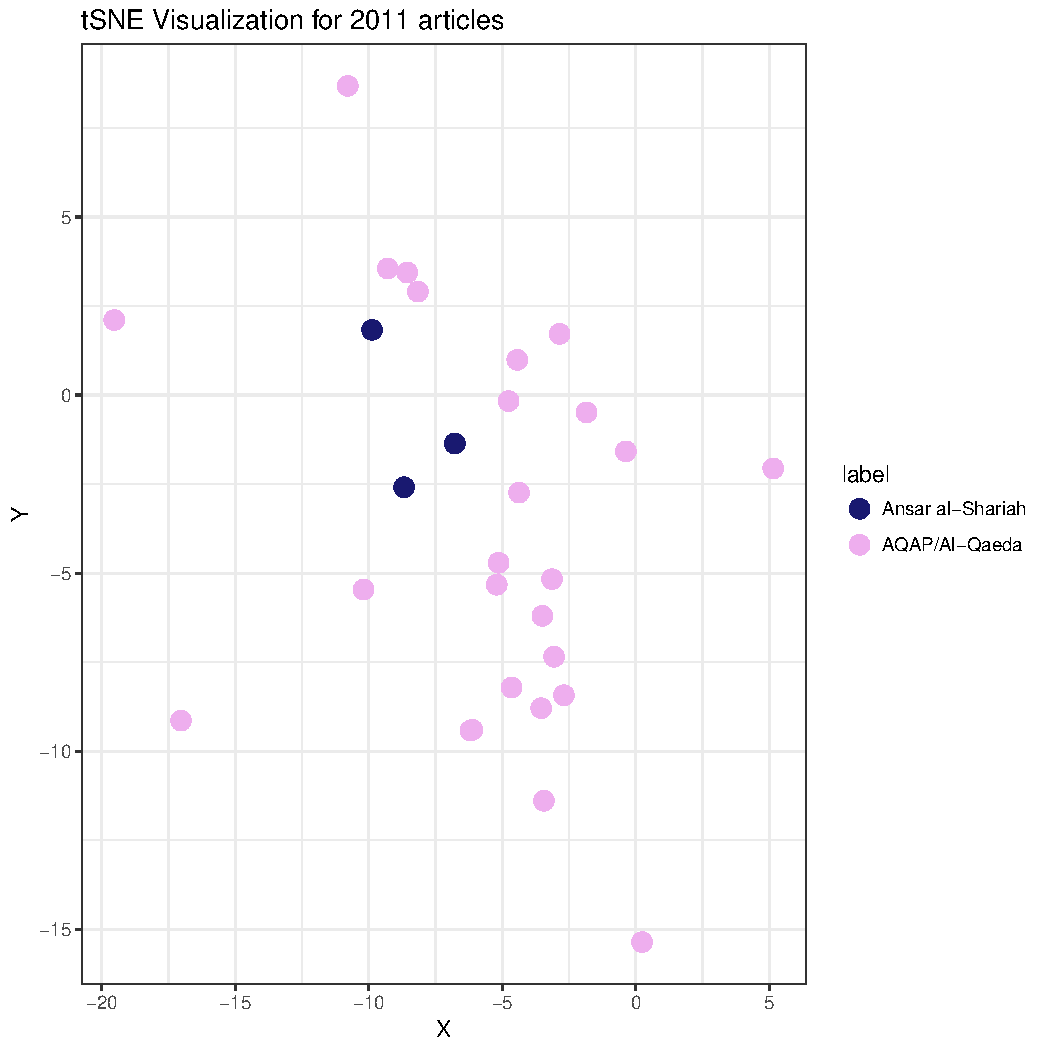
\includegraphics[width=.45\columnwidth]{./Pictures/2011sunnis_testData_tSNEDimRed.pdf}&
    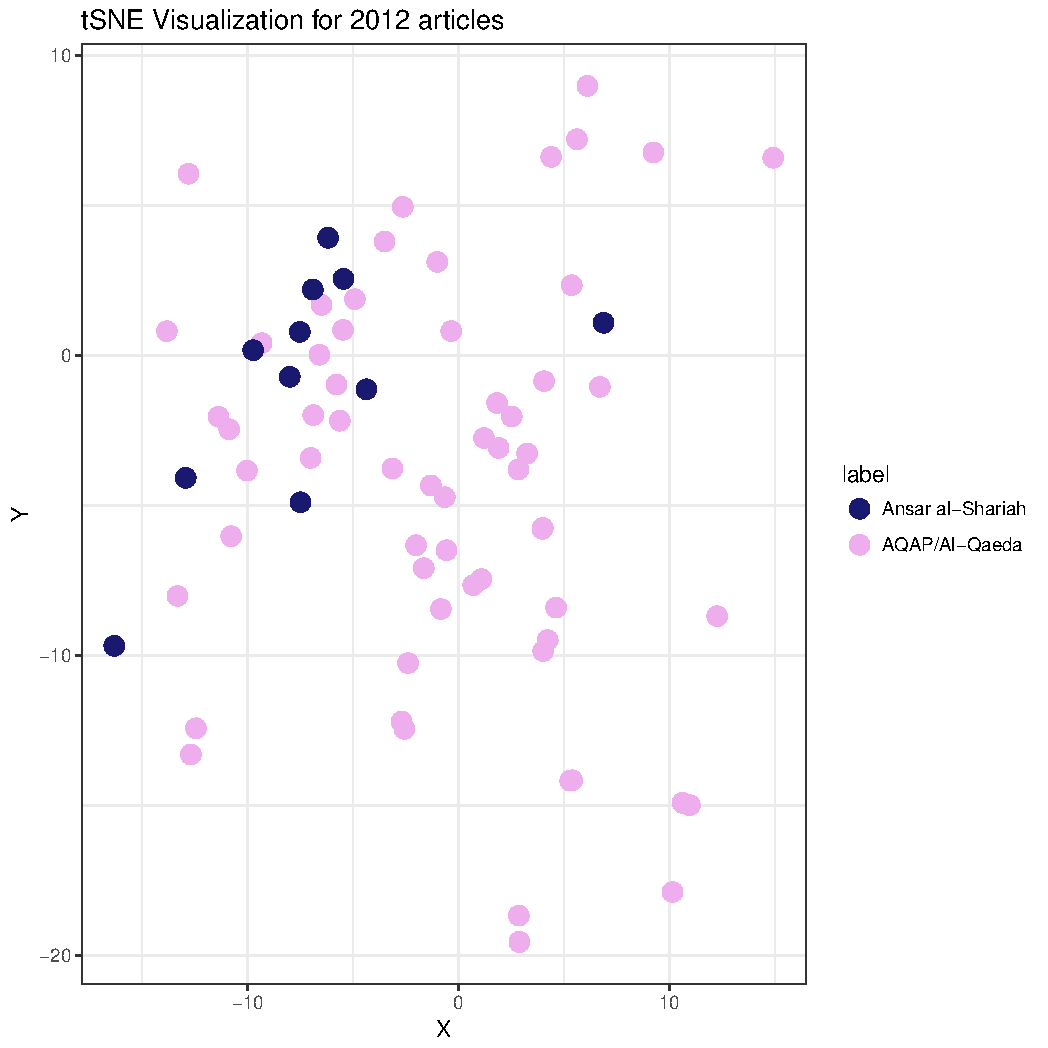
\includegraphics[width=.45\columnwidth]{./Pictures/2012sunnis_testData_tSNEDimRed.pdf}\\
    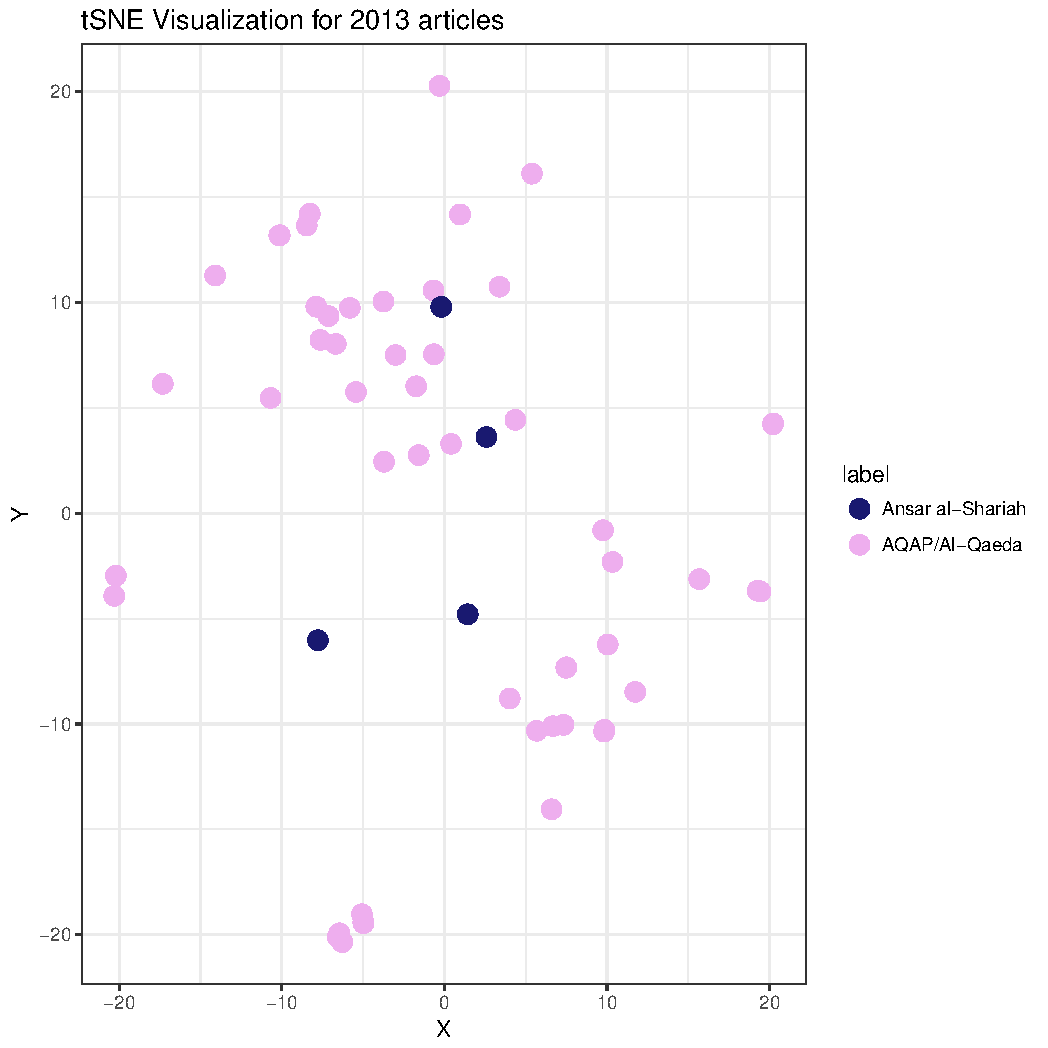
\includegraphics[width=.45\columnwidth]{./Pictures/2013sunnis_testData_tSNEDimRed.pdf}&
    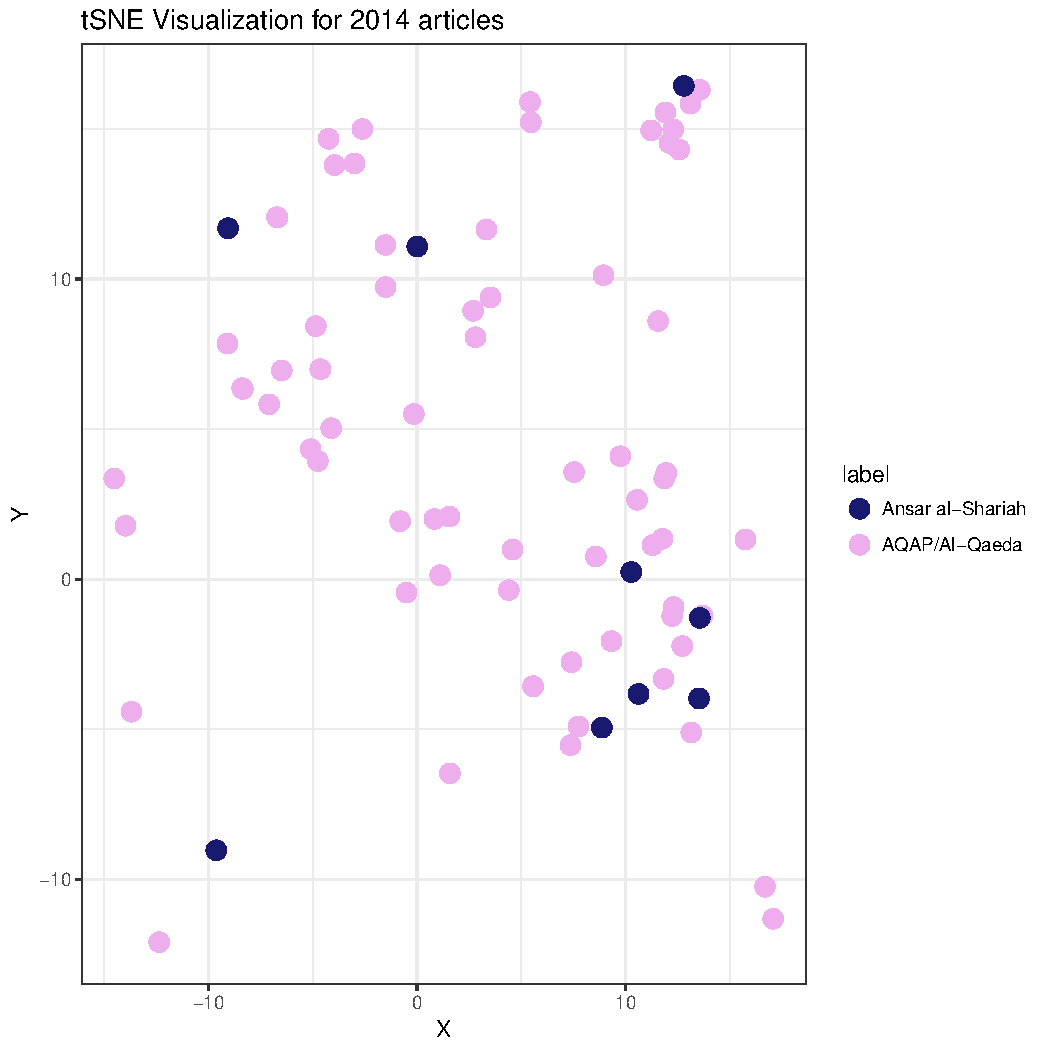
\includegraphics[width=.45\columnwidth]{./Pictures/2014sunnis_testData_tSNEDimRed.pdf}\\
  \end{tabular}
  \caption{tSNE Visualization Sunni Groups, 2011-2014}
  \label{fig:tsne-sunnis}
\end{figure}
\end{center}

\subsection{Random Forest Parameter Selection}

The random forest classifier used the randomforest() method from the
randomForest R package. The specification used the development data as training data, and the validation data as a test set, with story label as the classifier to predict. The confusion matrix for the training data is featured in the full text, while the confusion matrix for the training data appears below in Figure~\ref{tab:ref-conf-train}, followed by the classification results on the test data, in Figure~\ref{tab:ref-conf-test} .

The model grew 500 trees, from which is generated a proximity measure for each document. The variable importance plot was generated after extracting the variable importance measure and plotted using the varImpPlot() method native to randomForest. As the only predicted categories for the stories were AQAP and Houthi\/Ansarallah, the interpretation that
the random forest was identifying Houthi stories based on widespread description of the Shia group as a rebellion while the AQAP activities are more typically described as militant activity.

\begin{table*}[ht]
 \centering
 \begin{tabular}{rrrrr}
   \hline
  & AAS & AQAP/Al-Qaeda & Houthi & Class Error \\
   \hline
 Ansar al-Shariah & 0.00 & 24.00 & 2.00 & 1.00 \\
   AQAP/Al-Qaeda & 4.00 & 240.00 & 3.00 & 0.03 \\
   Houthi/Ansarallah & 0.00 & 7.00 & 152.00 & 0.04 \\
    \hline
 \end{tabular}
 \caption{Random Forest Confusion Matrix, Training Data}
\label{tab:ref-conf-train}
 \end{table*}
 
 
 \begin{table}[ht]
 \centering
 \begin{tabular}{rrrrr}
   \hline
  & AAS & AQAP/Al-Qaeda & Houthi & Class Error \\
   \hline
 Ansar al-Shariah & 0.00 & 6.00 & 3.00 & 1.00 \\
   AQAP/Al-Qaeda & 0.00 & 48.00 & 19.00 & 0.28 \\
   Houthi/Ansarallah & 0.00 & 14.00 & 25.00 & 0.36 \\
    \hline
 \end{tabular}
\caption{Random Forest Confusion Matrix, Test Data}
\label{tab:ref-conf-test}
 \end{table}
  
 
\begin{figure}
\begin{center}
\begin{tabular}{c}
  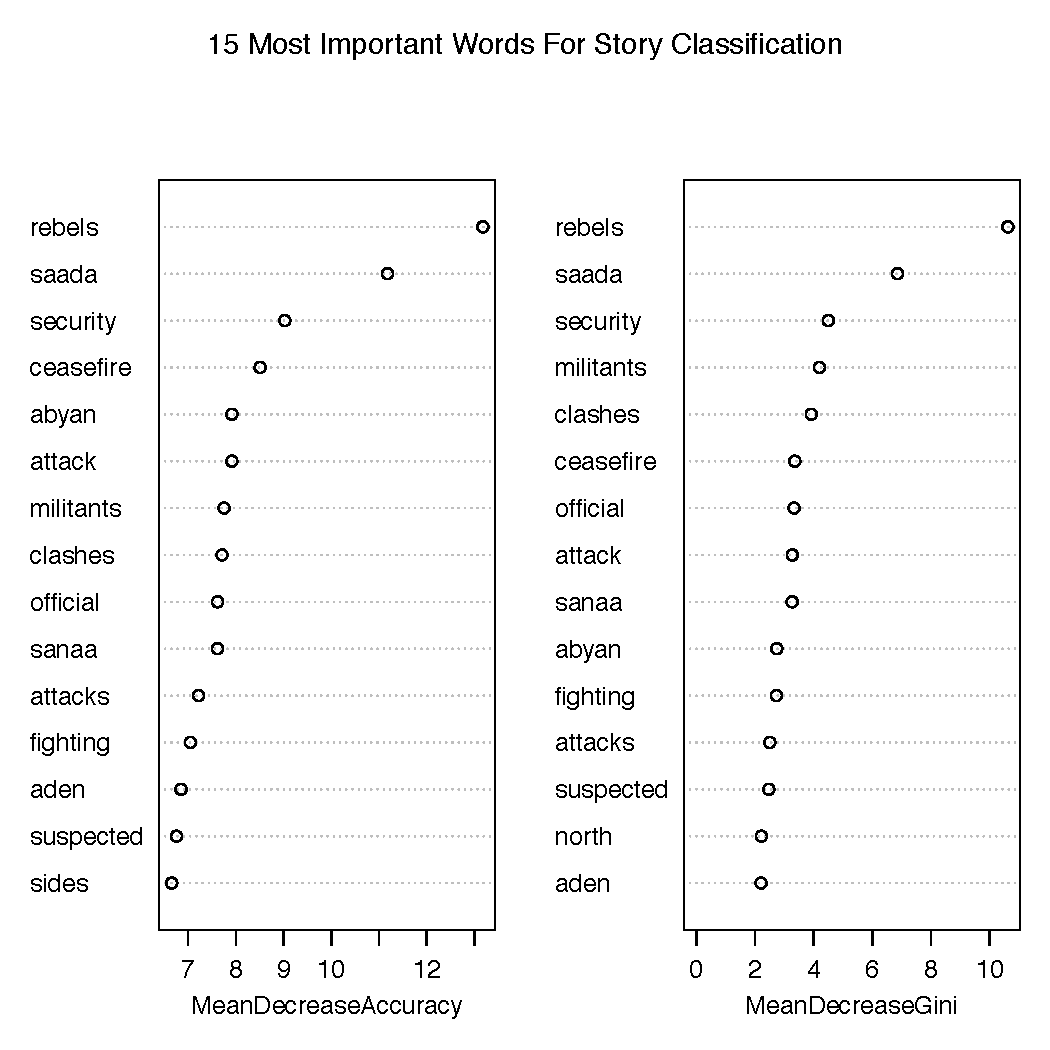
\includegraphics[width=5.00in]{./Pictures/randomForestRes.pdf}\\
\end{tabular}
\caption{Important Words for Classification}
\label{fig:rf-impt}
\end{center}
 \end{figure}

A second version of the random forest model estimated the model only on Ansar al-Shariah and AQAP stories. As with the full data, this
model failed to predict any stories for the Ansar al-Shariah
label. However, it did predict two AQAP-labeled stories as being
likely Ansar al-Shariah stories. These stories were an August 3, 2014
story about a clash between al-Qaeda militants and police forces and a
December 17, 2014 story about a car bomb carried out against Yemeni
police officers. Notably, both stories were one of the 11 stories from
Xinhua News that used the names AQAP and Ansar al-Shariah
interchangeably.

One advantage of the random forest approach to classifying text is that the features
used for classification are also terms in the document, which provide
interpretable insights into what words drive separation among stories
in the data. The fifteen most important words for the random forest
classification---after removing stopwords that describe or name the
active group--- suggest that the reason for the clean split
across the Sunni and Shia movements lies in framing. The list of these
terms, ranked in order of their importance for decreasing the
classifier accuracy (left) and importance for decreasing homogeneity
in the final nodes of the classification (right), can be seen in
Figure~\ref{fig:rf-impt}. The importance of \say{rebels} as the top term
for both accuracy and Gini coefficient is revealing: indeed in the
texts, Houthis are consistently described as \say{rebels} while the Sunni fighters are
frequently presented as \say{militants.}  After the rebel/militant
split, words that describe the location of operations and military occupations are, unsurprisingly, important classifiers:  Aden, Saada and Sanaa are
regions associated with Houthi territorial gains, while Abyan is more
closely linked to AQAP and Ansar al-Shariah
activities.

\subsection{Principle Component Analysis}

Another view of the separation among the stories is shown in
Figure~\ref{fig:rf-pca1}, which uses a principle component analysis (PCA) to
plot proximity of stories, as measured by the proportion of times that
individual stories are in the same terminal
node~\autocite{jones2015exploratory}.  This reaffirms the takeaway from
the confusion matrix: Houthi stories are distinct from AQAP stories,
but Ansar al-Shariah stories contain enough words in common with AQAP
stories that the two are difficult to distinguish via the random
forest's iterated decision trees.

\begin{figure}
\begin{center}
\begin{tabular}{c}
 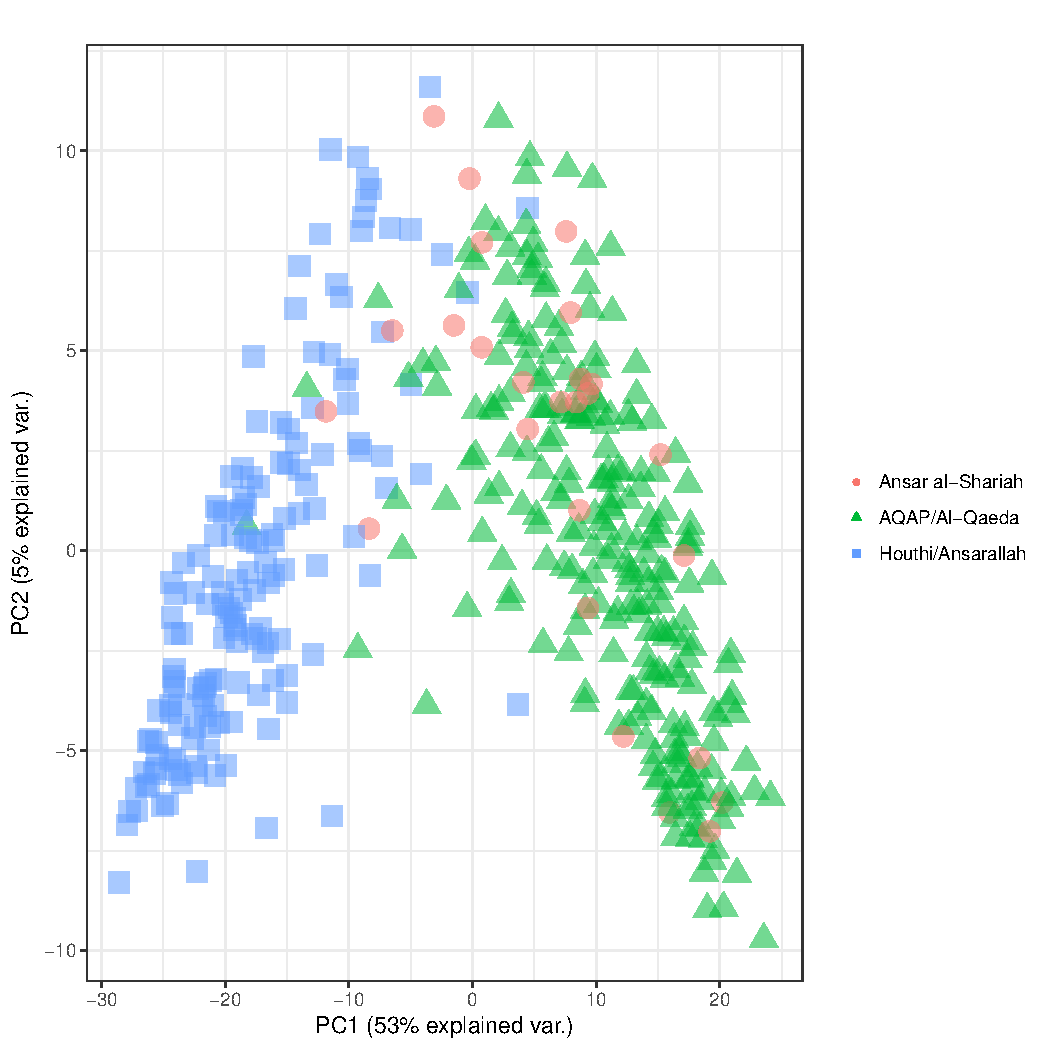
\includegraphics[width=5.00in]{./Pictures/pca_proximityRF.pdf}
\end{tabular}
\caption{PCA Visualization of Group Classification}
\label{fig:rf-pca1}
\end{center}
 \end{figure}

The principle component analysis presentation was done using the
extract\_proximity() and prcomp() methods from the edarf R
package. The proximity extraction categorizes document proximity as
the proportion of times that two observations are in the same terminal
node across each estimated tree. This generates an NxN matrix of
location similarities.  This proximity is visualized using a principle
components analysis of the proximity matrix, implemented in the edarf package.

\subsection{SVM Specification}

The support vector machine classification was developed using the
ksvm() method from the kernlab R package. I used the ``development''
data as a training set and the ``validation'' data as the test set,
with ``label'' as the classification attribute to predict and the
words from each term document matrix as the features used in the
classification.
The kernel specified was the radial basis function (RBF) Gaussian
kernel via kernlab's ``rbfdot'' implementation. The RBF kernel is
defined as:$K(x,x\prime)=$exp$(-\frac{||x-x\prime||^{2}}{2\sigma^{2}})$. This
kernel is based on squared Euclidean distance between feature vectors
for each document, and thus is amenable to interpretation as distance
between the documents. The svm carried out a 3-fold cross-validation
on the test set, and used the resulting model to predict category
assignment in the test (validation) set. In the analysis presented in
the paper, each class was given a weight of 1.  The paper reports
predicted probability of label assignment.

Given the imbalance in the data, I developed two additional versions of
the SVM model, subsetting the  development-validation data subset to include only AQAP and Ansar al-Shariah stories. One of these replicated the
original support vector machine with an equal weighting on each
possible class and one of which assigned class weights to the
labels in the 90-10\% distribution of AQAP and Ansar al-Shariah
stories.  Results of these two models were similar to the model
presented in the paper: given the words in
the news stories as features, the SVM does not distinguish Ansar
al-Shariah stories from AQAP stories.

Figure~\ref{fig:svm-mis} provides a closer look at whether the
support vector machine's confidence in whether to assign stories to
Ansar al-Shariah or AQAP change over time. Ideally, support for the
transformation theory would indicate the SVM assigning increasing weight to the Ansar
al-Shariah label for news stories about AQAP activities as AQAP
members push the group to engage with local concerns.  The plot
focuses on stories with a true label of AQAP and depicts the predicted
probability that an article would be assigned to the label of Ansar
al-Shariah given that it is a story about AQAP actions (red) as well as the
SVM's confidence in the classification for AQAP (blue) for the 144
stories in the test set. As the SVM consistently predicts all AQAP and
Ansar al-Shariah stories for AQAP, the expected probability of
assignment to Ansar al-Shariah remains constant at approximately
$p=.15$. The classification predictions provide mixed support for the
expectation that an influx of local members should increase the
difficulty of assigning group labels: although the SVM's confidence in
predicting the AQAP label becomes more variable over time, the
predicted probabilcde fg
issignmentcde fg
sar al-Shariah remains
constant over the time period

\begin{figure}
\begin{center}
\begin{tabular}{c}
  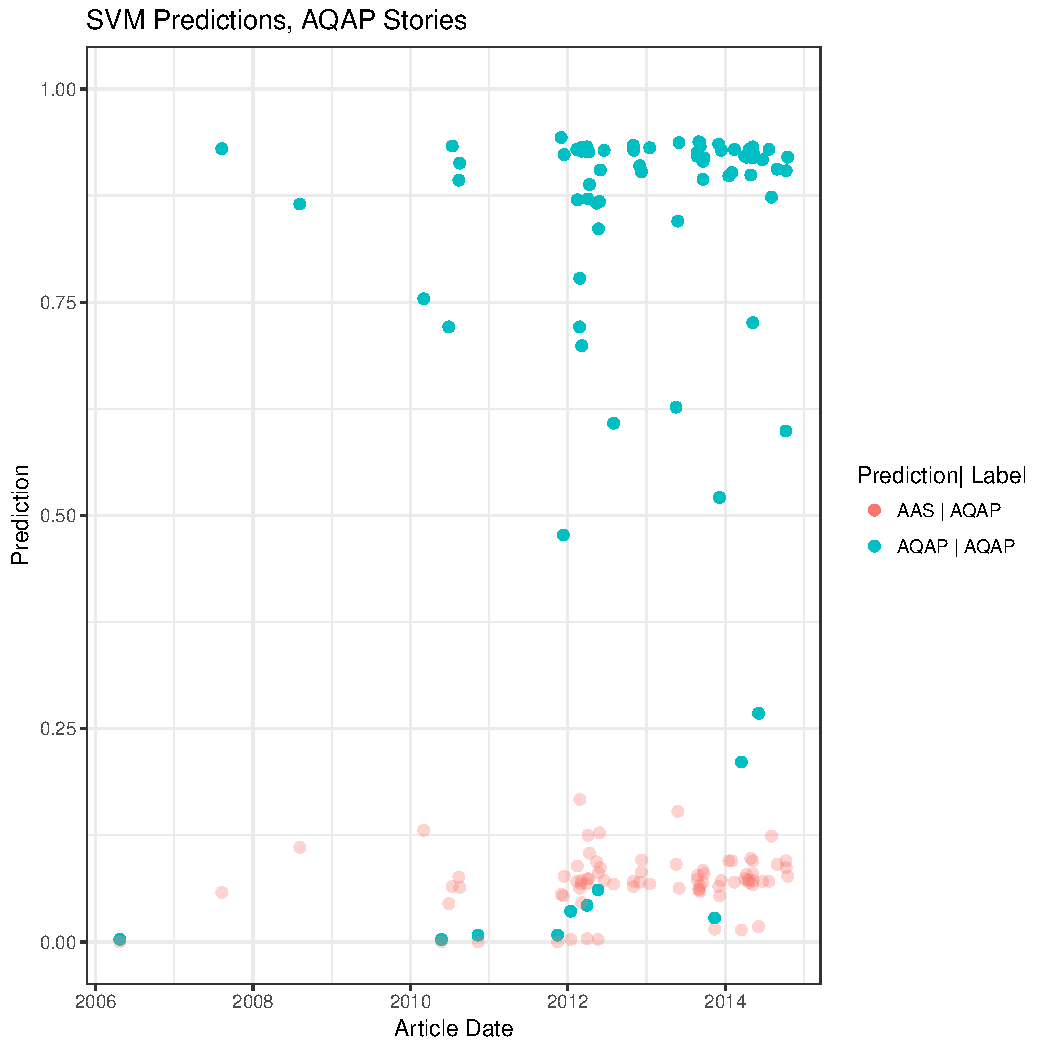
\includegraphics[width=5.00in]{./Pictures/PredictedProbabilities_AQAPPreds.pdf}\\
\end{tabular}
\caption{SVM Predictions Over Time For AQAP Stories}
\label{fig:svm-mis}
\end{center}
\end{figure}

\section{Structural Topic Model}

The three STM models are based on a corpus of 1353 documents, spanning October
25, 2005 through September 21, 2016. Approximately 500 documents are
associated with as-Sahab. A histogram of the distribution
of can be seen in Figure~\ref{fig:hist}. 

\subsection{Document Pre-processing}

I focus on media released online to jihadi media platforms and
outlets.  Preprocessing removed words that occurred in fewer than two or more 70\%
of the documents in the corpus.\footnote{In the AQAP corpus, there was
no change to the number of tokens in the corpus for an upper bound
threshold between 70-95\%. I evaluated coherence and exclusivity at
an upper threshold of 50\%, but did not find results that would
suggest either a coherence or exclusivity benefit from the additional
reduction in corpus size.}

\begin{figure}
\begin{center}
  \begin{tabular}{c}
    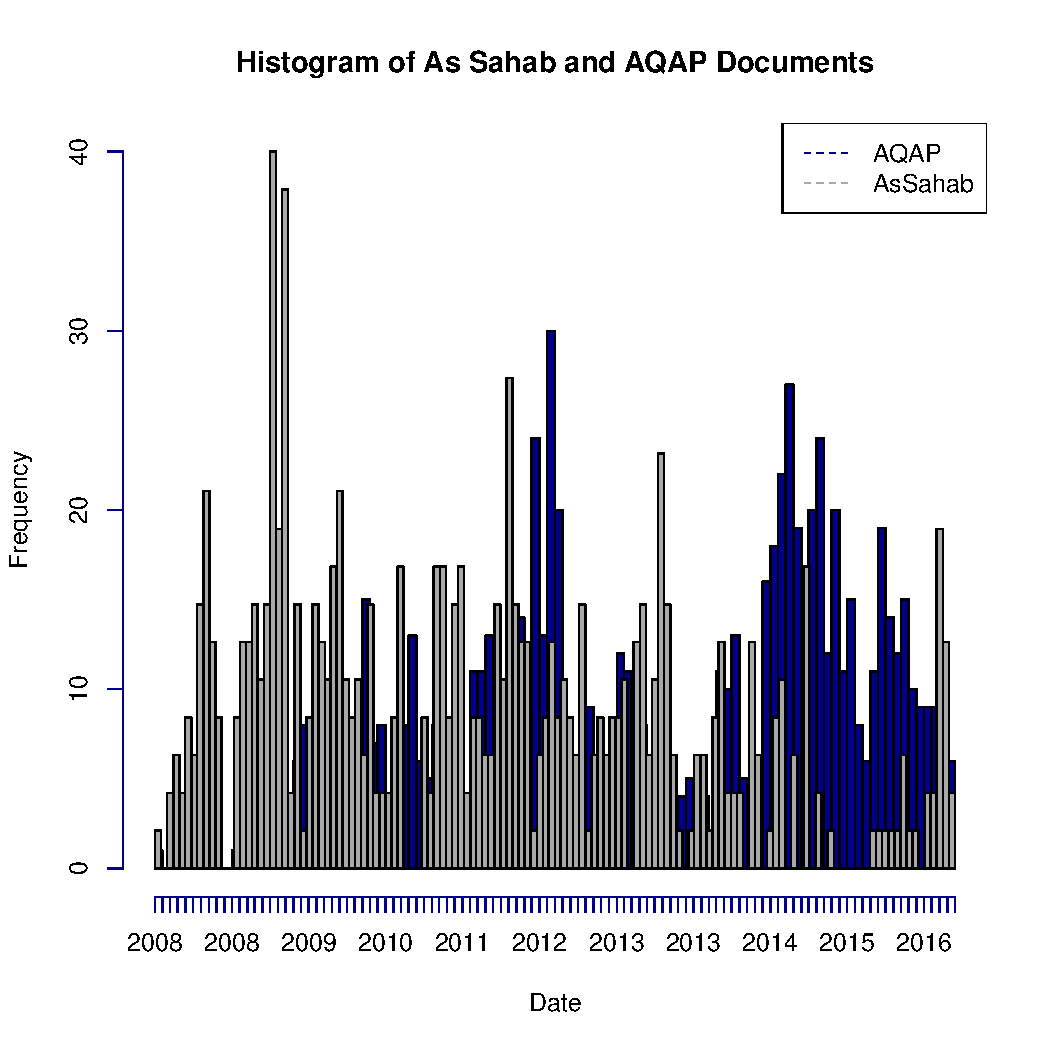
\includegraphics[width=5.00in]{./Pictures/histofAQAPandAS.pdf}
  \end{tabular}
  \caption{Distribution of AQAP and AQC Materials}
  \label{fig:hist}
\end{center}
\end{figure}

Models One, Two, and Three each use time as a covariate. The time
variable is expressed in the data as a running counter of days from
the oldest document in each corpus. Thus, the date of the oldest
document is given as 1 and the \say{day} of each subsequent document is
modeled as the numer of days between the first date and the date of
the individual document. These dates are linked to the                                                           
  translation date rather than release date as the former can be                                            
  accurately pinpointed for each document in the corpus. For the vast                                       
  majority of the corpus, the translation date closely coincides with                                       
  the date that the document was released to online jihadi media outlets. The precision                     
  of release dates contained in the original Arabic text can vary                                           
  according to type of document: communiques are typically dated                                            
  to a specific day, while strategy documents or promotional magazines                                      
  can be dated with a day, a month, or even a season. Thus, for                                             
  consistency, the date covariate is linked to translation date.

\subsection{Model Selection}
Topic models rely on the user to prespecify a number topics for the
algorithm to search for. However, this parameter fundamentally influences the themes that will be
identified in the documents.  For models one and two, I selected the number of topics by doing a
sweep of model specifications with 10 to 30 topics. I selected a
topic number that performed best on both semantic coherence and
exclusivity.\footnote{Ideally, the selected number of topics would
  have relatively high exclusivity and semantic coherence. I often
  faced a trade-off between the two. When determining the trade-off, I
  prioritized semantic coherence over exclusivity. The exclusivity bands were, overall, narrow while
coherence varied substantially.} After this process, a model with 18 topics
appeared to present the greatest gains to semantic coherence without
trading off exclusivity. Moreover, the 18-topic model identified
topics that were particularly substantively coherent. 

For the joint model, after comparing the semantic
coherence-exclusivity trade-off for models across a sweep from 10
to 40 topics, I set the number of topics to discover at
34. The increase of topics reflects the expectation that the two
organizations are already rhetorically distinct, and so the joint
corpus should require more topics. Specifically choosing an output
that doubled the number of topics slightly penalized semantic
coherence over a model with fewer topics, but allowed for a more
precise comparison of topics between each group. 

As topic models are, by nature, non-deterministic, each
implementation of a given model will produce slightly different
results. Thus, after selecting the number of topics for the STM to
identify, I ran each model specification ten times to create a range of
possible output models for analysis. I compared the average
semantic coherence and exclusivity for each of the models. For each of
the three models below, I found that the averages within each
ten-model set were nearly identical. To avoid biasing my results by
selectively choosing the output that best confirms my theoretical expectations, I chose
which specific models to analyze by maximizing average coherence
and exclusivity metrics. As no model clearly dominated the
coherence-exclusivity trade-off, I assigned a relatively stronger
weighting to semantic coherence when selecting a specific iteration to
present. I then selected a model to present before qualitatively evaluating any of the topics. This
decision was intended to avoid bias in choosing how to prioritize
coherence gains against exclusivity losses.\footnote{A plot of average
semantic coherence and exclusivity scores is available upon request.} 
 
Finally, after selecting which model to present, I evaluated the
remaining models to ensure that the output was consistent across the
set of ten results for each model. In particular, I verified general
agreement on the thematic content identified across the runs.

% \subsection*{Choice of topic number}
%% [Ed note: commented out until I figure out if k=17 here was a typo
%% or if I had a reason to say that K=17 had highest semantic
%% coherence, but I went with k=18]

% I set the number of topics with reference to balancing semantic
% coherence, exclusivity, and held-out likelihood of models varying
% values of K. Exclusivity was in a narrow range for both the AQAP and
% As-Sahab corpus, so I placed most weight on semantic coherence.

% For AQAP documents, k=17 is clear winner for high semantic coherence,
% but has among lowest exclusivity. Next best are the 34, 36, 39
% cluster. They have highest exclusivity and in top 9/40 coherence. 

% \begin{center}
% \begin{table}
%   \begin{tabular}{cc}
%     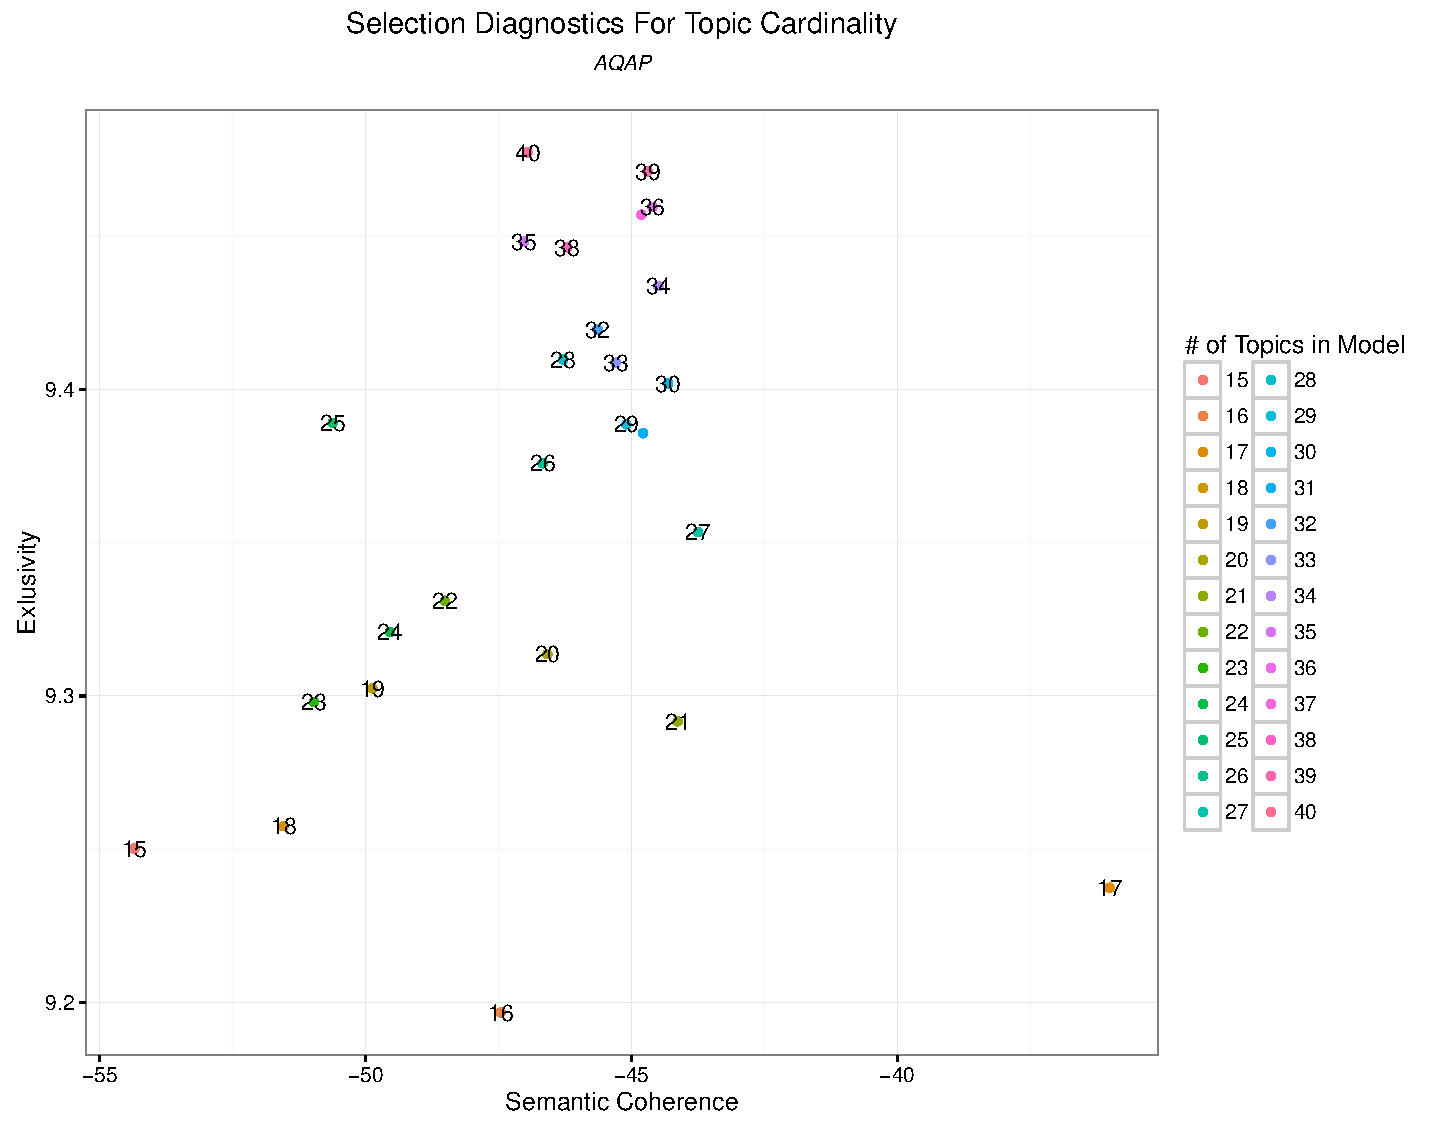
\includegraphics[width=3.00in]{aqapAQAPKSelectSummary.pdf}&
%     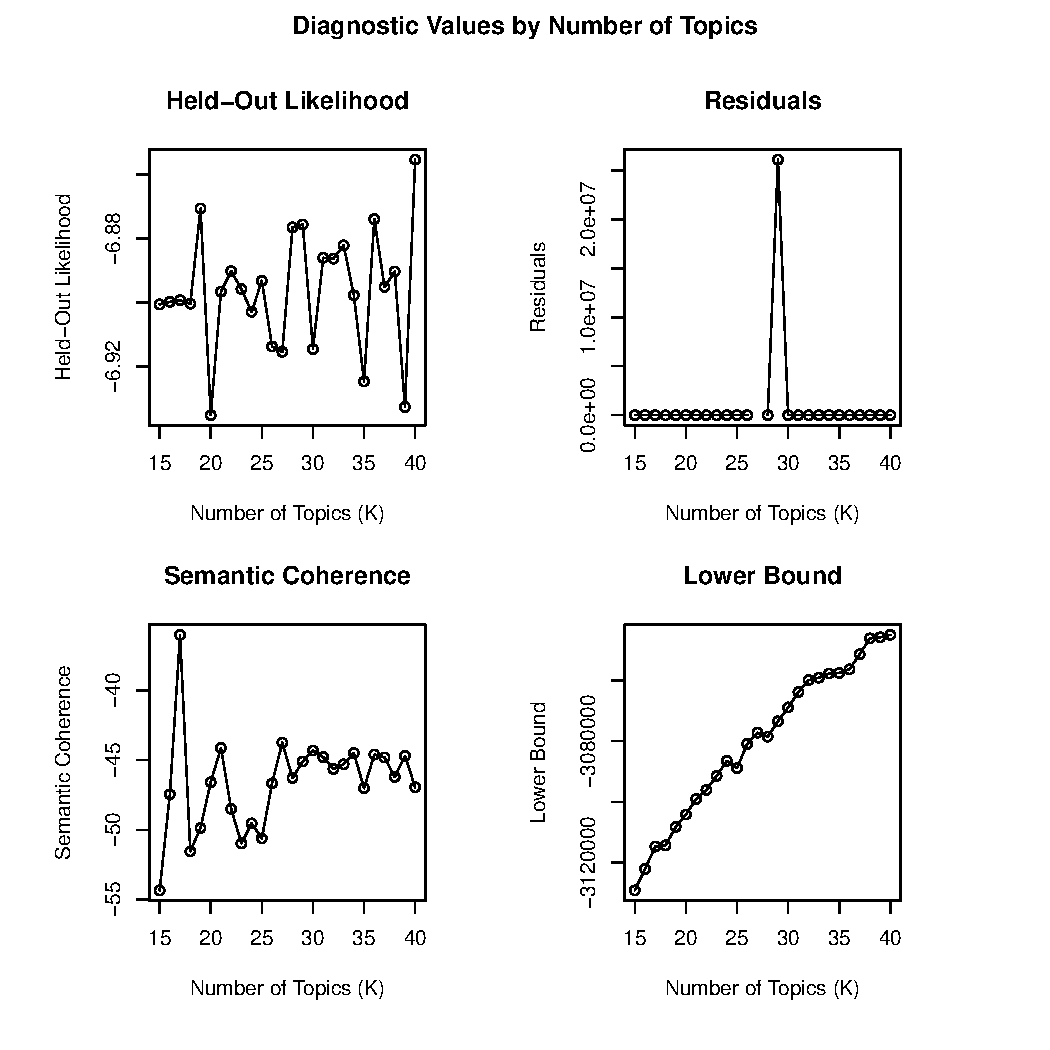
\includegraphics[width=3.00in]{aqapbaseDiagnosticPlot.pdf}
%   \end{tabular}
%   \caption{Model Diagnostics for AQAP Corpus}
%   \label{tab:aqapdiag}
% \end{table}
% \end{center}

% For as-Sahab, k=15, 16, 17, and 18 are all tightly clustered at the
% highest end of coherence. The range for exclusivity is particularly narrow, so I put most of the selection weight on semantic coherence.
% \begin{center}
% \begin{table}
%   \begin{tabular}{cc}
%     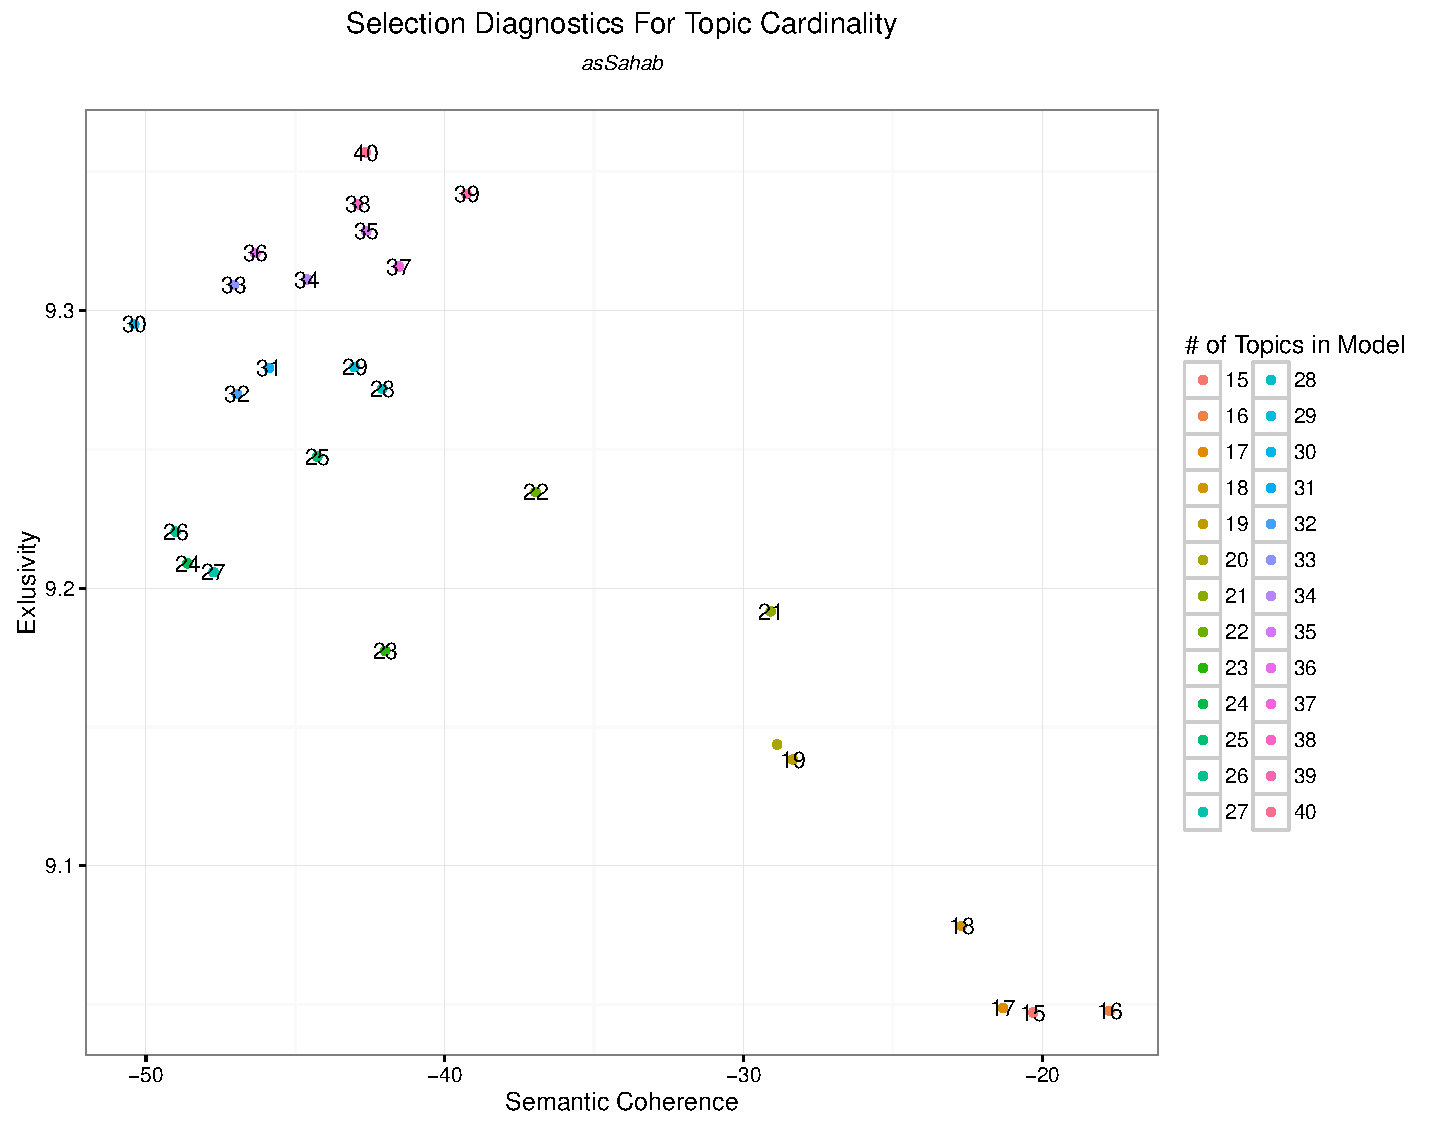
\includegraphics[width=3.00in]{asSahabAQAPKSelectSummary.pdf}&
%     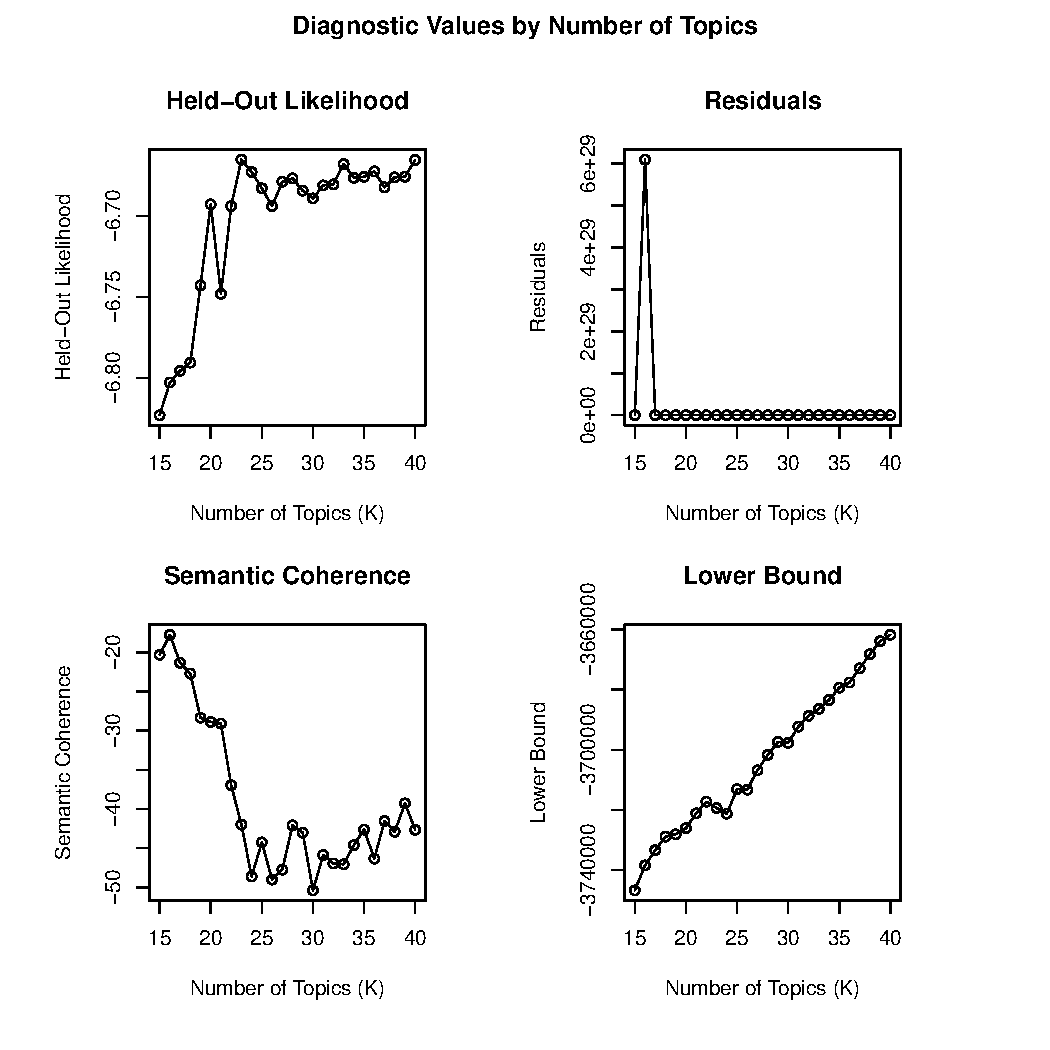
\includegraphics[width=3.00in]{asSahabbaseDiagnosticPlot.pdf}
%   \end{tabular}
%   \caption{Model Diagnostics for as-Sahab Corpus}
%   \label{tab:asbdiag}
% \end{table}
% \end{center}

%% \underline{Additional topics in Model One}\\

%% The two remaining Yemen-centric topics are topics 3 and 11. Topic 3, labeled as the
%% ``Southern Yemen'' topic strongly relates to AQAP's 2011 seizure of territory in the
%% south of the country during the 2011 Revolution. The topic rises in
%% prominence while the organization controlled territory in 2011 and
%% 2012, and then quickly recedes as an expected thematic topic.  As
%% such, the topic is a useful indicator that the STM model identified
%% are reflective of underlying events.  footnote{The third Yemen-related
%%   topic, loosely named the ``US in Yemen'' topic, does not has as
%%   clearly interpretable thematic structure as do the other three
%%   Yemen-centric topics, and so is not presented here.}

 Figure~\ref{fig:civsandfactions} depicts the expected proportion
of the transnational jihadi topics presented according to
time.\footnote{For interpretability, the x-axis is labeled by year. The model was
  estimated according to the number of days from the start of the
  document corpus.}  The y-axis represents the expected proportion of
each document dedicated to each topic. For context, I added four
vertical lines marking important dates identified above. From left to right, the
lines represent: the al-Majalah airstrike on December 17, 2009; the start of
the Yemeni Revolution on January 27, 2011; the death of Usama bin
Laden on May 2, 2011; the end of the first Obama Administration on
January 19, 2012; and the Houthi takeover of Sanaa on September 21, 2014.

\subsection{Local Conflict Topics}

The \say{Local Conflict} cluster is comprised of four STM-identified topics. The topics are unified by a shared focus on people and places local to Yemen, as well as tactical terms that suggest military operations.  

Within the cluster, specific topics are internally unified by their focus. One topic, which I have named \say{Southern Yemen} is characterized by geographic references to Abyan Governorate, which was held by Islamic militants in 2012.  Another, the \say{Local Targets} topic has a geographic focus on Hadramawt Governorate in Central Yemen and makes frequent references to specific operational behaviors and targets. The \say{Houthis} local topic combines frequent temporal references with military terms, a combination that is indicative of claims of military operations.

Figure~\ref{fig:houthisLT} shows temporal trends in the expected proportion of the corpus dedicated to each of the four topics in the \say{Local Topics} cluster. Notably, the \say{Houthi} and \say{Southern Yemen} topics closely track then-current events. Each topic rises in prevalence in the corpus corresponding to the dates of the respective military offensives. Moreover, that the unsupervised topic model \say{discovered} the military offensives provides a useful source of external validity for the 18-topic model.

\begin{figure*}
\begin{center}
\caption{Changes over time to attention dedicated to local topics}
  \label{fig:houthisLT}
  \begin{tabular}{c}
    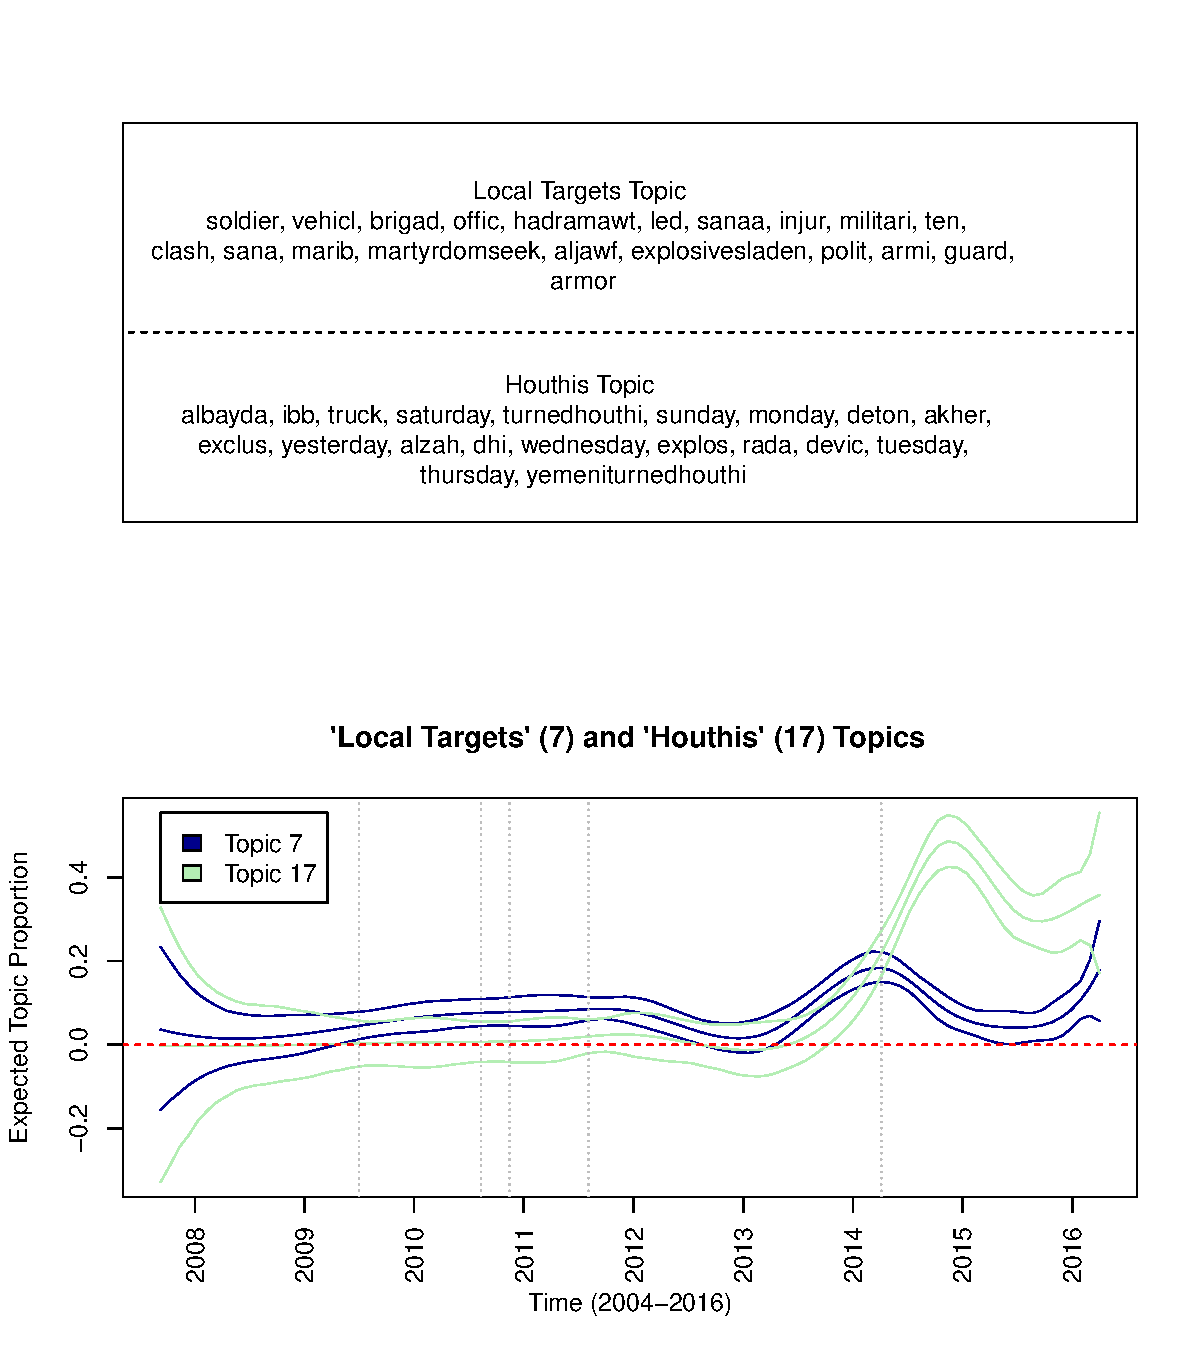
\includegraphics[width=.65\columnwidth]{./Pictures/HouthiandLT_UT7_K18.pdf}\\
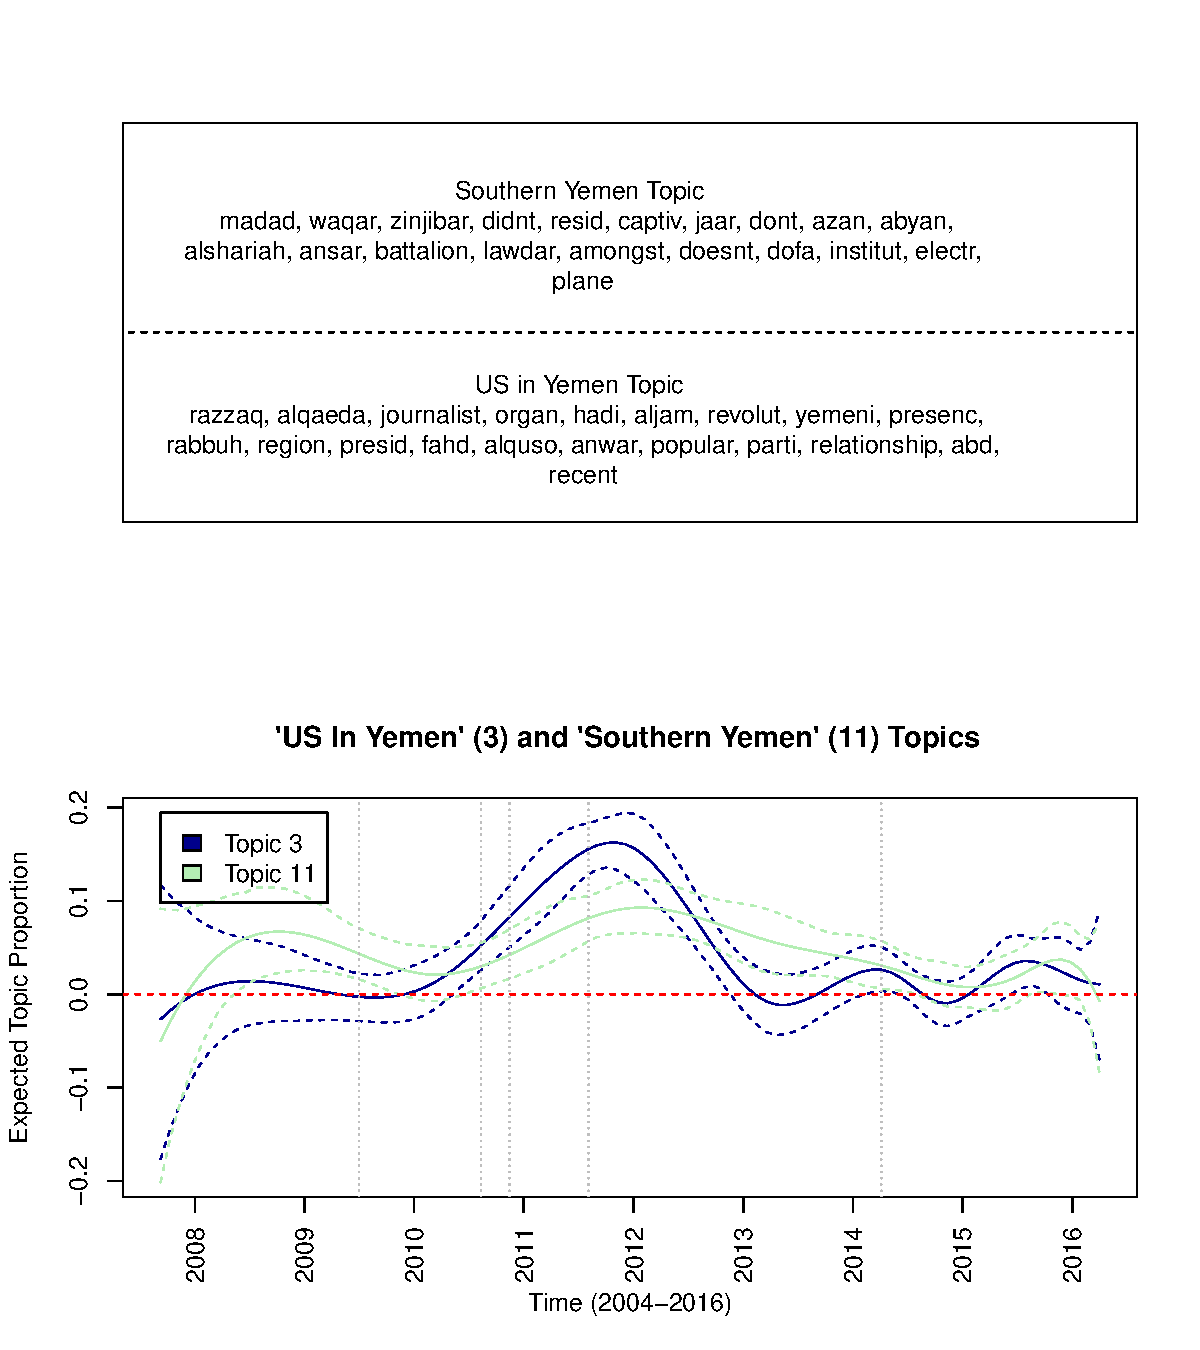
\includegraphics[width=.65\columnwidth]{./Pictures/AASAndMiscYemen_UT7_K18.pdf}\\
  \end{tabular} 
\end{center}
  \end{figure*}

\subsection{Transnational Jihadi Topics}

The first topic is dedicated to naming groups that
the jihadi worldview considers global enemies of Islam. I term this
the \say{Clash of Civilization} topic, as the FREX words reflect a
pervasive jihadi doctrinal focus on fighting a perceived global
alliance of Jews and Christians who are attempting to subjugate
Muslims. The \say{Clash of Civilizations} topic begin to decline after
about 2009, an important benchmark, as the year saw a number of
high-profile drone strikes that caused widespread resentment.  This
decline may speak to the bottom-up transformation of interest
described above: if localizing rhetoric was driven by top-down
marketing decisions, and the group turned away from global jihadi
branding to capitalize on domestic frustrations, we might
expect to see a sharper decline in the topic during 2009.

The second transnational jihadi topic, topic 15, centers on words that indicate an attempt to sooth conflicts among and between jihadi communities and other Muslim groups. Thus, I label this topic \say{Jihadi Factionalism.} FREX words for the topic feature words used when attempting to recapture ideological legitimacy. %The topic
%declines throughout 2009 and 2010, 

The third topic presented in Figure~\ref{fig:civsandfactions}, the
\say{Jihadi Revolution} topic, is centered around concepts used to
incite for overthrow of secular governments and implementation of an
Islamic theocracy. Such revolutionary rhetoric is central to the
transnational jihadi view of themselves as a vanguard of social and
political revolution.  The topic declines briefly after the first inflection
point, then rises from mid-2010 through mid-2013 before taking a more
dramatic downturn at the second point. One reason why the \say{Jihadi
Revolution} topic may not reflect the theorized \say{transnational}
topic decline may be that the 2011 Yemeni Revolution increased the
group's interest in presenting itself as a viable alternative to the
Yemeni state.

The fourth transnational topic in Figure~\ref{fig:civsandfactions} is
topic 2, labeled \say{Demise of al-Saud.} The topic is
focused on Saudi-centric themes, and references to Saudi officials and the state's repression
of jihadi dissidents. The topic is largely stable at an expected prevalence of
approximately 5\%  throughout the time period.  I code this topic as a
\say{transnational} topic because the Saudi-lead intervention in the Yemeni
civil war, \say{Operation Decisive Storm,} was launched only in 2015 and so for the
majority of the dates analyzed, Saudi Arabia was an external target.

\begin{figure*}
\begin{center}
\caption{Changes over time to attention given to global jihadi topics }
  \label{fig:civsandfactions}
  \begin{tabular}{c}
    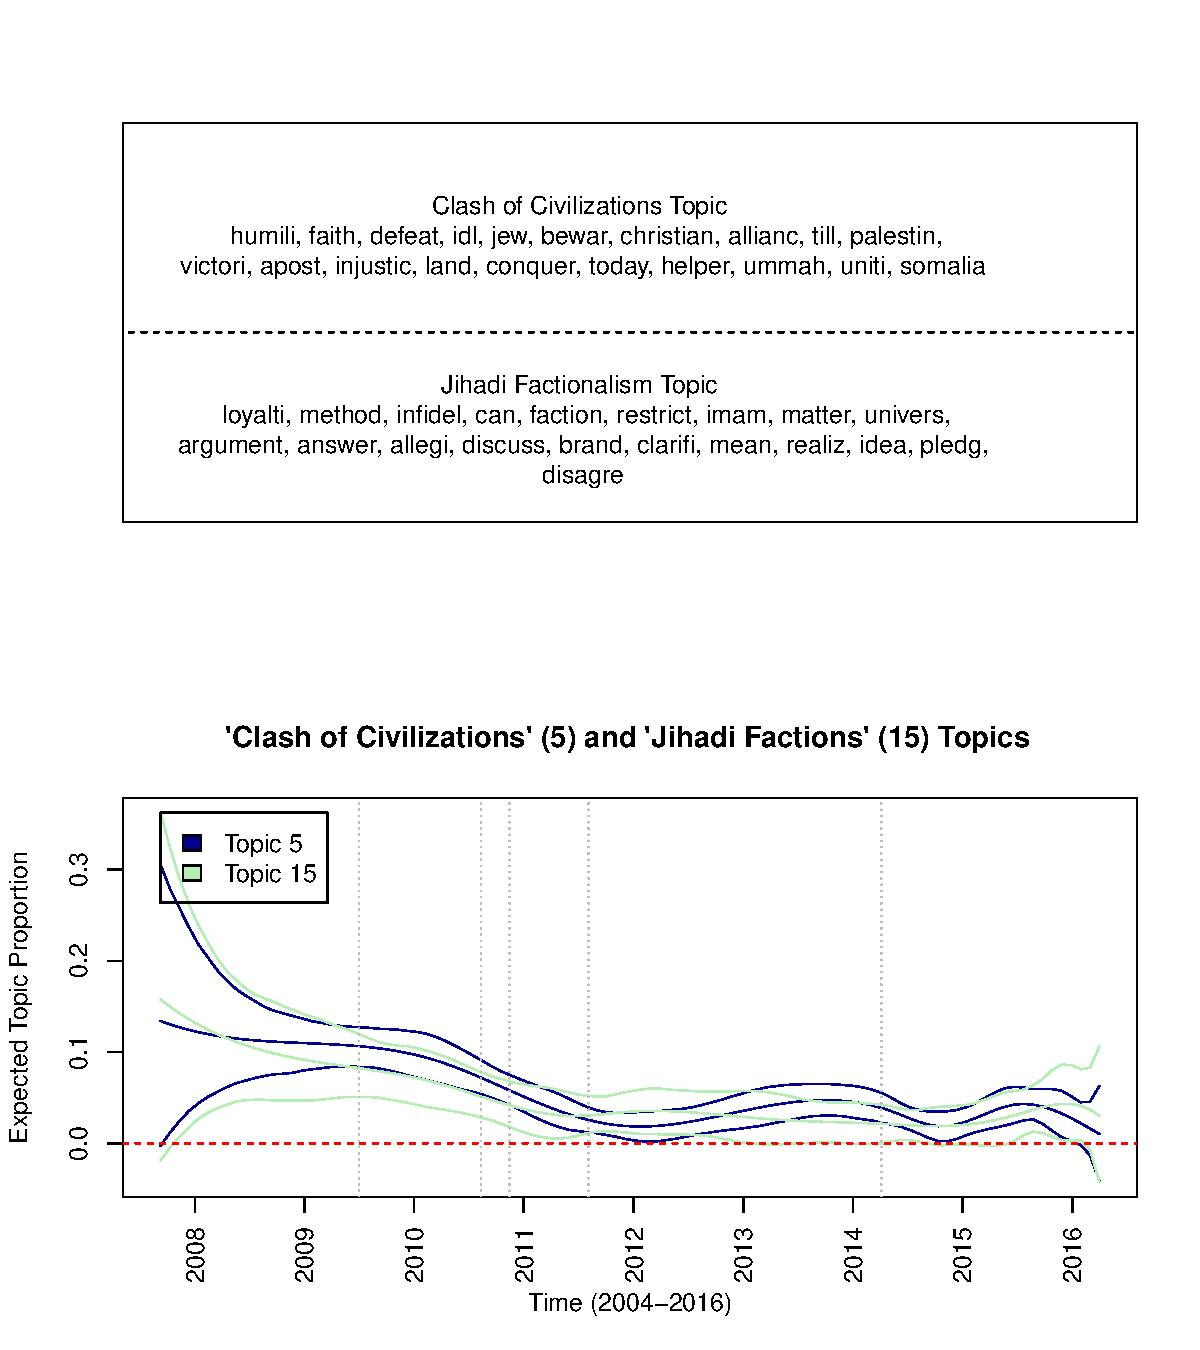
\includegraphics[width=.65\columnwidth]{./Pictures/ClashFactions_UT7_K18.pdf}\\
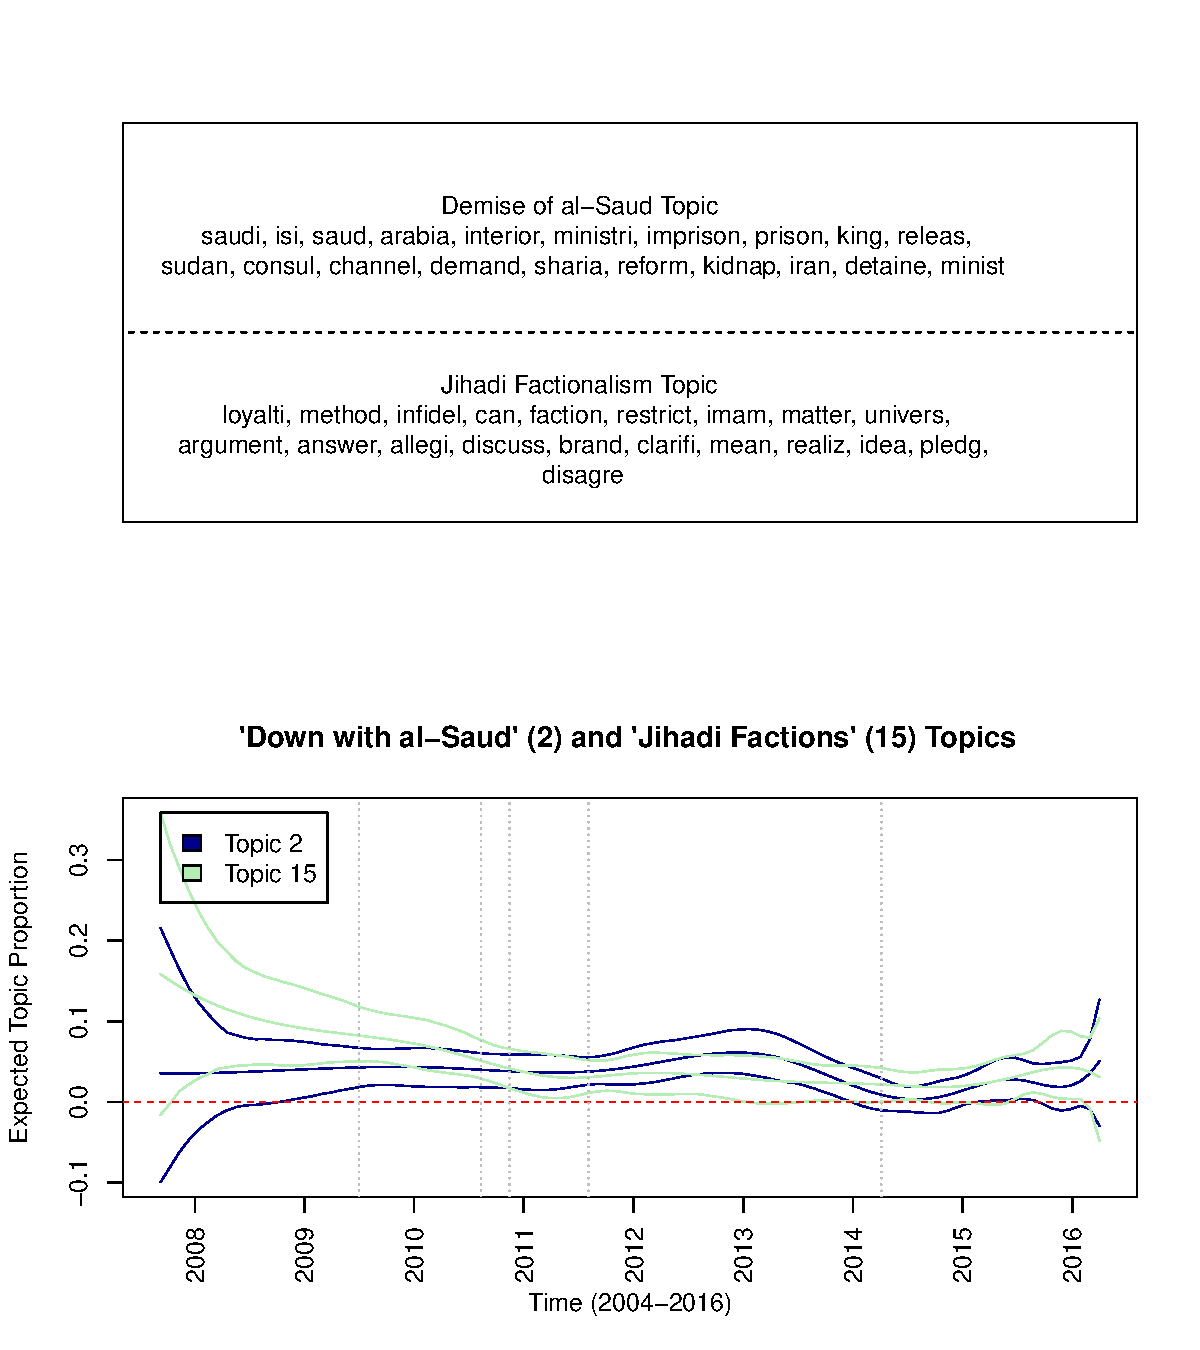
\includegraphics[width=.65\columnwidth]{./Pictures/TransJihadiAlt_UT7_K18.pdf}\\
  \end{tabular} 
\end{center}
  \end{figure*}
